\section{Neutrino Oscillations in Matter}


\subsection{Matter Interactions and MSW Effect}


\begin{frame}{Matter Interaction}


% \begin{tcolorbox}[title=PLACEHOLDER]
% SHOULD ADD IN WHY MATTER INTERACTION IS LIKE THIS.
% \end{tcolorbox}



\begin{tcolorbox}[sidebyside]
% \begin{figure}[ht]
\centering
% \begin{minipage}[b]{0.45\linewidth}
\centering
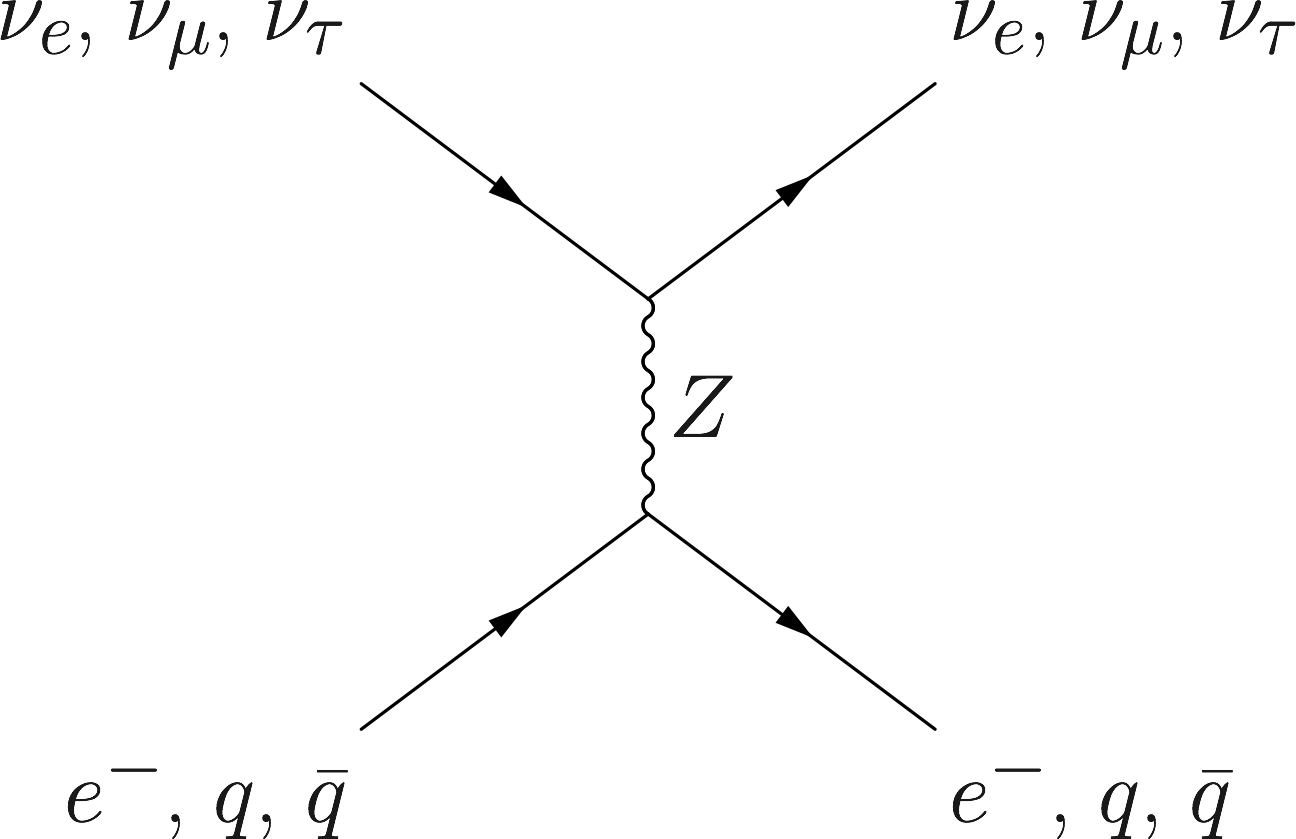
\includegraphics[height=0.32\textheight]{assets/neutral-current.png}

\color{black}Neutral current interaction between $\nu_{\mathrm e}$, $\nu_{\mu}$, $\nu_{\tau}$,
and $e^{-}$.
% \end{minipage}%
\tcblower
% \begin{minipage}[b]{0.45\linewidth}
\centering
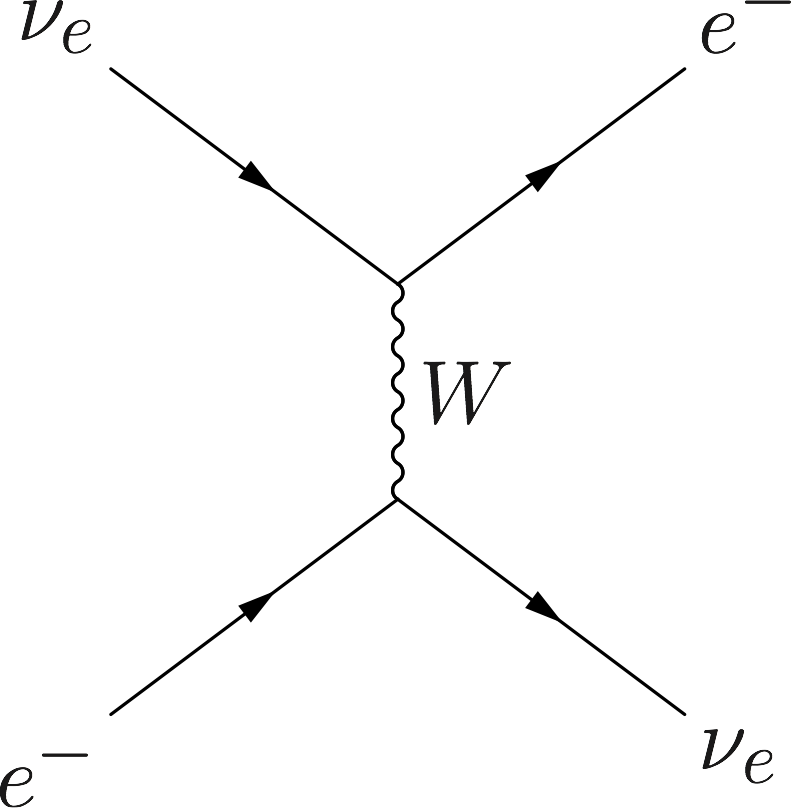
\includegraphics[height=0.32\textheight]{assets/charged-current.png}

\color{black}Charged current interaction between $\nu_{\mathrm e}$ and $e^{-}$
% \end{minipage}
% \end{figure}
\end{tcolorbox}


\end{frame}





% For every picture that defines or uses external nodes, you'll have to
% apply the 'remember picture' style. To avoid some typing, we'll apply
% the style to all pictures.
\tikzstyle{every picture}+=[remember picture]


% By default all math in TikZ nodes are set in inline mode. Change this to
% displaystyle so that we don't get small fractions.
\everymath{\displaystyle}







% For every picture that defines or uses external nodes, you'll have to
% apply the 'remember picture' style. To avoid some typing, we'll apply
% the style to all pictures.
\tikzstyle{every picture}+=[remember picture]


% By default all math in TikZ nodes are set in inline mode. Change this to
% displaystyle so that we don't get small fractions.
\everymath{\displaystyle}



\begin{frame}{Matter Interaction}
\setbeamercovered{invisible}

\tikzstyle{na} = [baseline=-.5ex]




\begin{itemize}
    \item[] Hamiltonian with matter interaction in flavor basis  (\color{white}$\omega_{\mathrm{v}}=\delta m^2 \big/ 2E$):
        \tikz[na] \node[coordinate] (n1) {};
\end{itemize}




\only<1->{
\begin{equation*}
    \mathbf{H} =
    \tikz[baseline]{
            \node[fill=blue!50,anchor=base] (t1)
            {$ \frac{\omega_{\mathrm{v}}}{2}\left( - \cos 2\theta_{\mathrm{v}} \boldsymbol{\sigma_3} + \sin 2\theta_{\mathrm{v}} \boldsymbol{\sigma_1} \right) $}
            }
            \tikz[baseline]{
            \node[fill=red!50, anchor=base] (t2)
            {$
            +\frac{\lambda(x)}{2} \boldsymbol{\sigma_3}
            $};
        }
\end{equation*}

}


\begin{itemize}
    \item \colorbox{blue!50}{Vacuum Hamiltonian}
        \tikz[na]\node [coordinate] (n2) {};
    \item \colorbox{red!50}{Matter interaction}
        \tikz[na]\node [coordinate] (n3) {};
    \item<1-> $\lambda(x) = \sqrt{2}G_{\mathrm{F}} n_{\mathrm{e}}(x)$
\end{itemize}





% Now it's time to draw some edges between the global nodes. Note that we
% have to apply the 'overlay' style.
\begin{tikzpicture}[overlay]
        \path[->]<1-> (n2) edge [bend right] (t1);
        \path[->]<1-> (n3) edge [bend right=20] (t2);
\end{tikzpicture}




\end{frame}





\begin{frame}{Matter Interaction}

\begin{align*}
    \mathbf H =& \colorbox{blue!50}{$ \frac{\omega_{\mathrm{v}}}{2}\left( - \cos 2\theta_{\mathrm{v}} \boldsymbol{\sigma_3} + \sin 2\theta_{\mathrm{v}} \boldsymbol{\sigma_1} \right) $}   \colorbox{red!50}{$ + \frac{\lambda(x)}{2} \boldsymbol{\sigma_3} $} \\
    \to &  \colorbox{blue!50}{$ \omega_{\mathrm v}\begin{pmatrix}
    - \sin 2\theta_{\mathrm v} \\
    0 \\
    \cos 2\theta_{\mathrm v}
\end{pmatrix} $}  \colorbox{red!50}{$ + \begin{pmatrix}
    0\\
    0\\
    - \lambda(x)
    \end{pmatrix} $} \\
    = &  \colorbox{blue!50}{$ \vec H_{\mathrm v} $}  \colorbox{red!50}{$ + \vec H_{\mathrm m}(x) $}
\end{align*}






\end{frame}




\begin{frame}{Matter Interaction}



\begin{columns}[T]
\begin{column}{0.5\textwidth}


\begin{figure}
    \centering
    \colorbox{white}{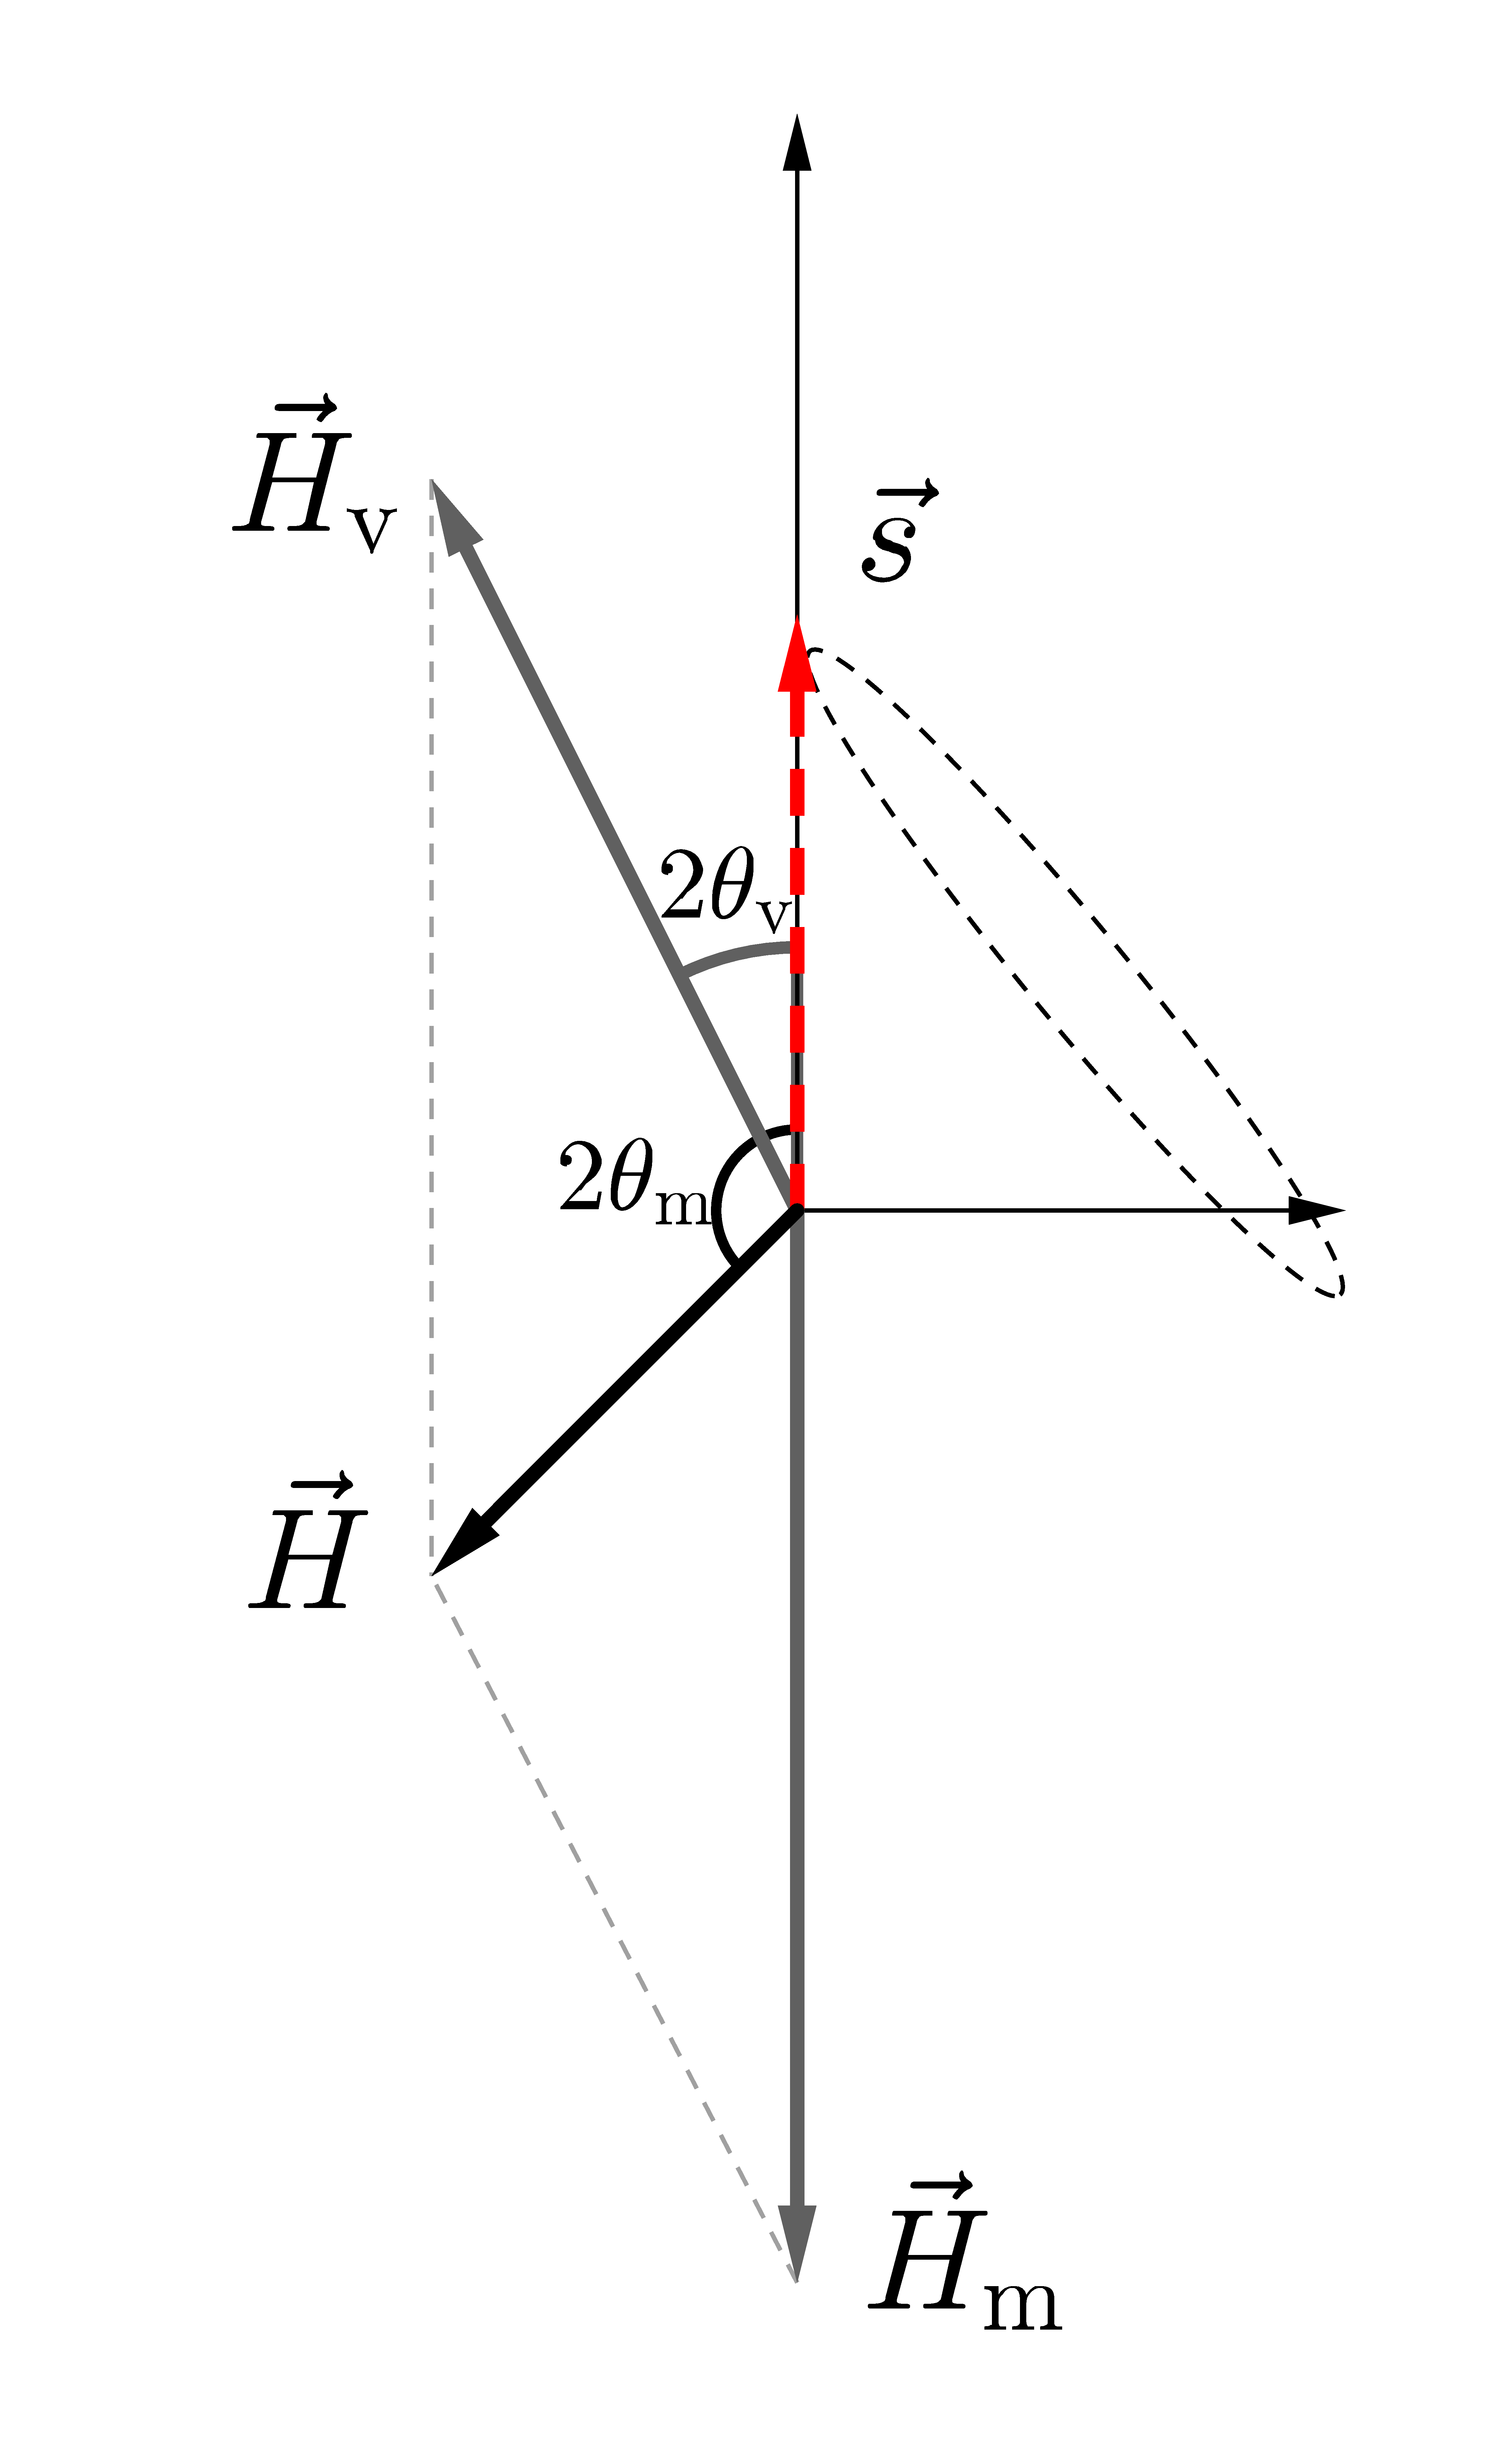
\includegraphics[width=0.9\textwidth]{assets/matter-effect-notsolarge-density}}
\end{figure}


\end{column}%
\begin{column}{0.5\textwidth}



Electron flavor survival probability

\begin{equation*}
P = \frac{1}{2} + s_3
\end{equation*}

Oscillation frequency in {\bf vacuum}:

\begin{equation*}
    \omega_{\mathrm v} = \lvert \vec H_{\mathrm v} \rvert
\end{equation*}


Oscillation frequency in {\bf matter}:

\begin{equation*}
    \omega_{\mathrm m} = \lvert \vec H \rvert
\end{equation*}

Flavor states and mass states in matter

\begin{equation*}
\begin{pmatrix}
\psi_e\\
\psi_\mu
\end{pmatrix} = \begin{pmatrix}
\cos \theta_{\mathrm m} & \sin\theta_{\mathrm m} \\
-\sin \theta_{\mathrm m} & \cos \theta_{\mathrm m}
\end{pmatrix}\begin{pmatrix}
\psi_{\mathrm L}\\
\psi_{\mathrm H}
\end{pmatrix}
\end{equation*}


\end{column}
\end{columns}

\end{frame}





\begin{frame}{MSE Resonance}


\begin{columns}[T]
\begin{column}{0.5\textwidth}



\begin{figure}
    \centering
    \colorbox{white}{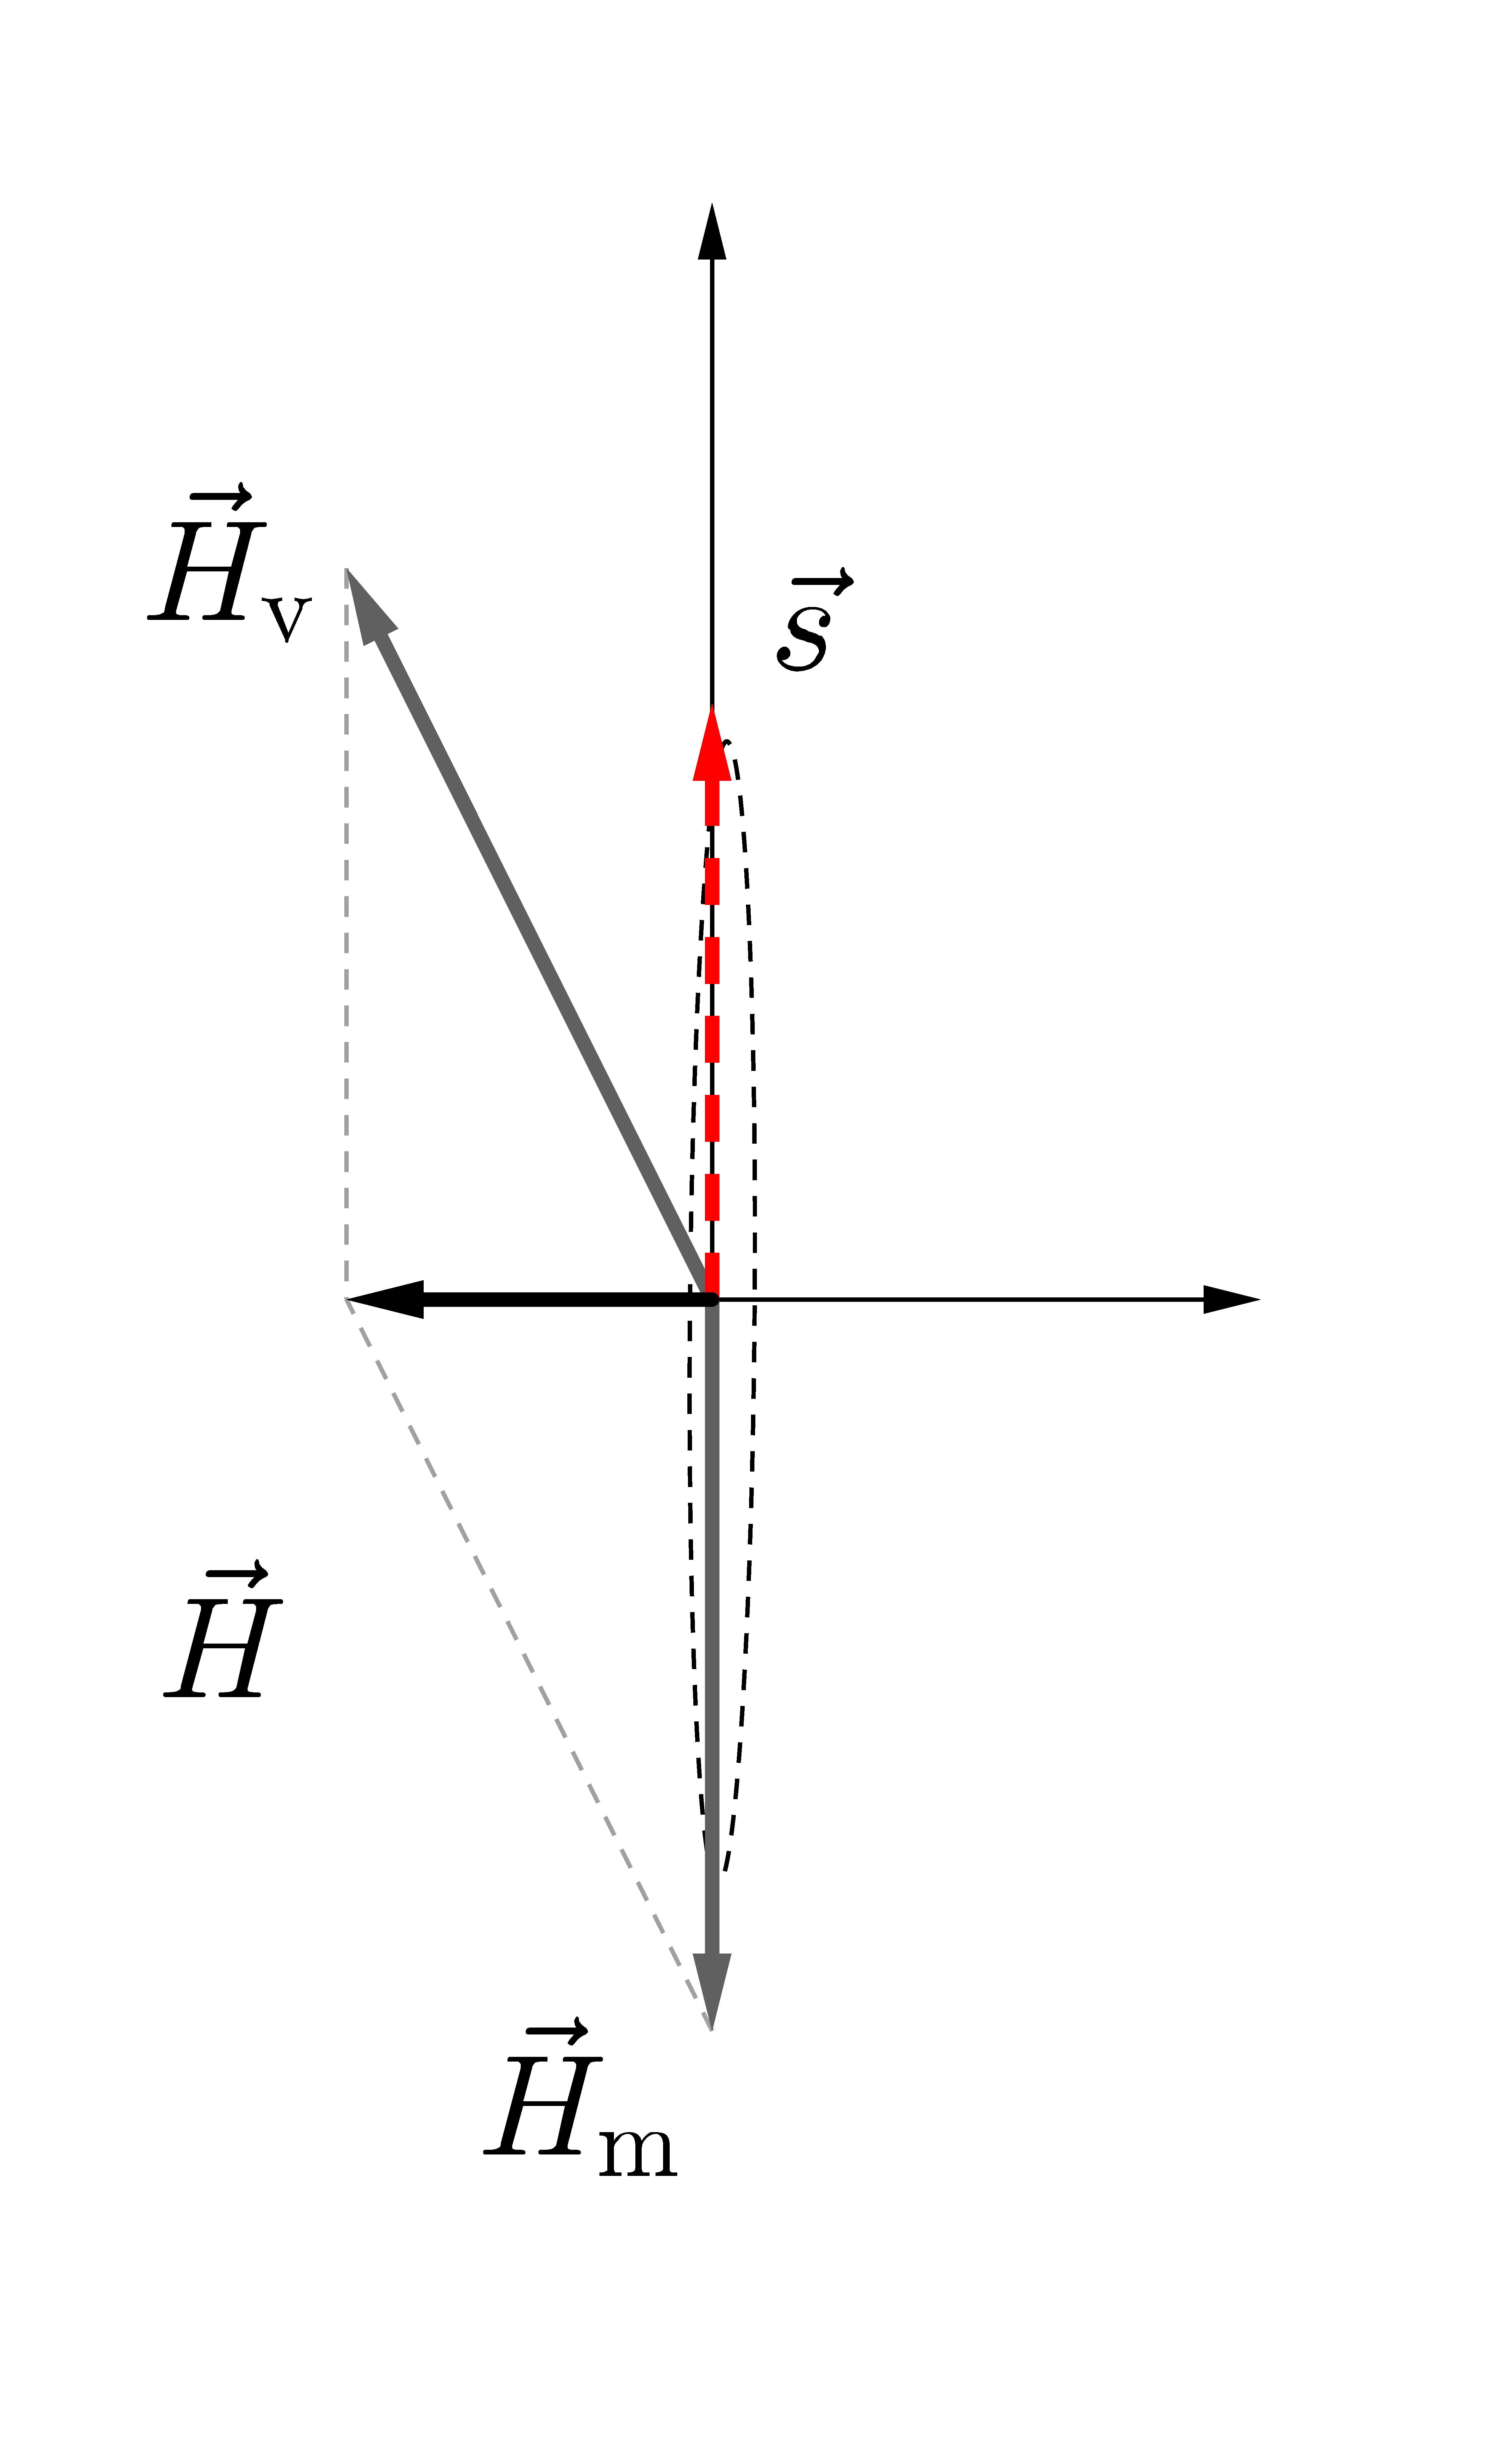
\includegraphics[width=0.9\textwidth]{assets/matter-effect-critical-density}}
\end{figure}


\end{column}%
\begin{column}{0.5\textwidth}



\begin{itemize}
\item
Maximum possible flavor transition probability amplitude
\item
MSW Resonance
\item
A specific matter density
\begin{equation*}
    \sqrt{2}G_{\mathrm F}n_{\mathrm e} \equiv \omega_{\mathrm v}\cos 2\theta_{\mathrm v}
\end{equation*}


\end{itemize}









\end{column}
\end{columns}







\end{frame}


\begin{frame}{MSW Effect}



\centering

\vspace{-1em}
Adiabatic matter density change

\begin{columns}[T]
\begin{column}{0.33\textwidth}

\begin{textblock*}{70pt}(50pt,47pt)
\small
Large density
\end{textblock*}

\only<2->{
\begin{textblock*}{70pt}(160pt,47pt)
\small
Lower density
\end{textblock*}
}
\only<3->{
\begin{textblock*}{70pt}(280pt,47pt)
\small
Low density
\end{textblock*}
}


\begin{figure}
    \centering
    \colorbox{white}{\includegraphics[width=0.7\textwidth]{assets/matter-effect-large-density}}
\end{figure}


\end{column}%
\begin{column}{0.33\textwidth}

\pause

\begin{figure}
    \centering
    \colorbox{white}{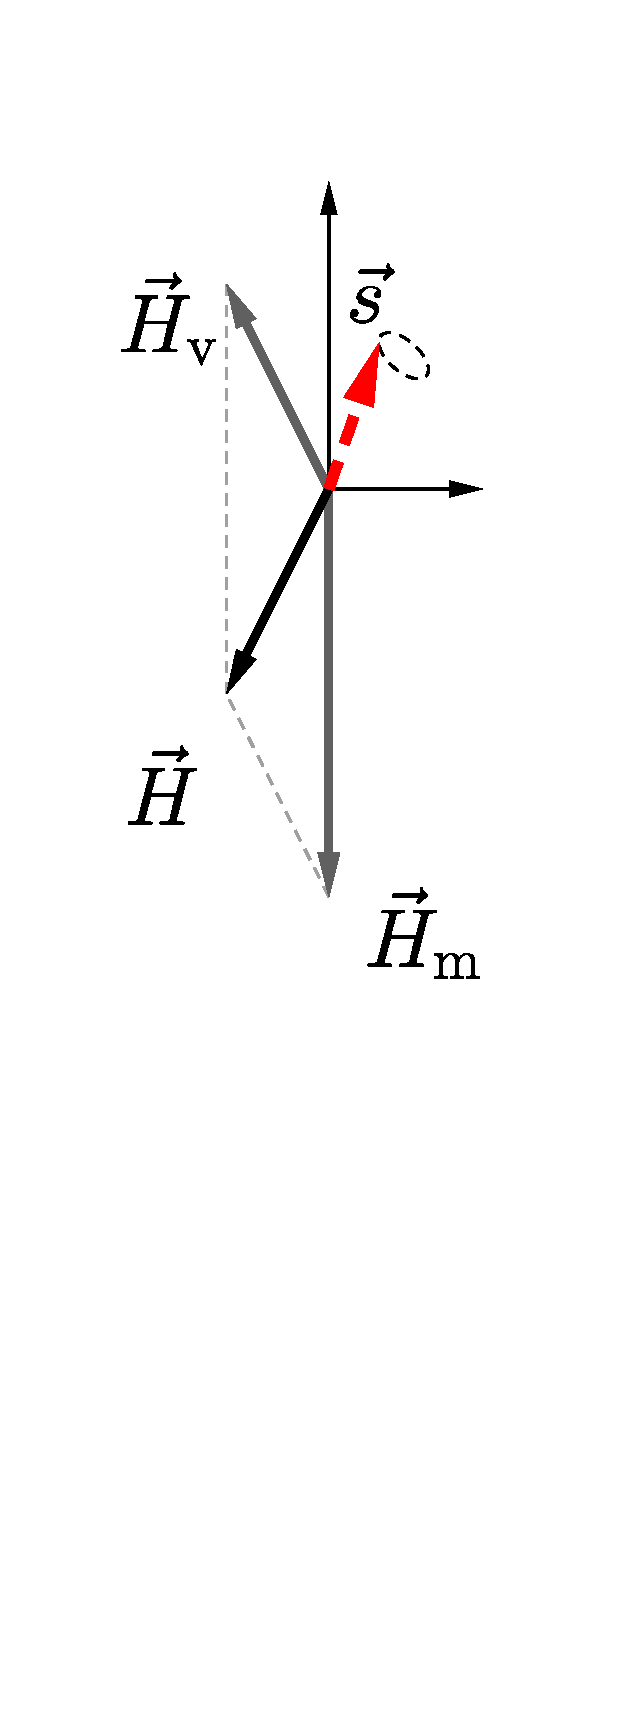
\includegraphics[width=0.7\textwidth]{assets/matter-effect-adiabatic}}
\end{figure}



\end{column}
\begin{column}{0.33\textwidth}

\pause

\begin{figure}
    \centering
    \colorbox{white}{\includegraphics[width=0.7\textwidth]{assets/matter-effect-adiabatic-3}}
\end{figure}



\end{column}
\end{columns}



\end{frame}



%%%%%%% MSW Effect %%%%%%%%%

%\subsubsection{Solar Neutrino Problem}
%
% \begin{frame}{Solar Neutrino Problem}
%
%
% \begin{figure}
%     \centering
%     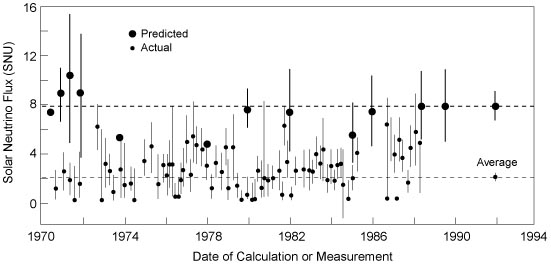
\includegraphics[width=0.9\textwidth]{assets/chlorine-detector-solar-neutrinos.jpg} %https://ase.tufts.edu/cosmos/print_images.asp?id=37
%     %https://ase.tufts.edu/cosmos/view_picture.asp?id=585
%     \caption*{Chlorine detector (Homestake experiment) results and theory predictions. SNU: 1 event for $10^{36}$ target atoms per second. Kenneth R. Lang (2010)}
% \end{figure}
%
%
% \end{frame}
%
%
% \begin{frame}{MSW Effect and Solar Neutrinos}
%
% % \setbeamercovered{invisible}
%
%
%
% \begin{equation*}
%     \mathbf{H} = \frac{\lambda(x) - \omega_{\mathrm v} \cos 2\theta_{\mathrm v}}{2} \boldsymbol{\sigma_3} + \frac{ \omega_{\mathrm v} \sin 2\theta_{\mathrm v}}{2} \boldsymbol{\sigma_1}
% \end{equation*}
%
%
% \begin{equation*}
% \begin{pmatrix}
% \ket{\nu_{\mathrm{L}}} \\
% \ket{\nu_{\mathrm{H}}}
% \end{pmatrix} =
% \begin{pmatrix}
% \cos\theta_{\mathrm m} & -\sin\theta_{\mathrm m} \\
% \sin\theta_{\mathrm m} & \cos\theta_{\mathrm m}
% \end{pmatrix}\begin{pmatrix}
% \ket{\nu_{\mathrm{e}}} \\
% \ket{\nu_{\mu}}
% \end{pmatrix}
% \end{equation*}
%
%
% \begin{equation*}
%     \mathbf{H}_{\text{matter-basis}} = -\frac{\omega_{\mathrm m}}{2}\boldsymbol{\sigma_3}
% \end{equation*}
%
%
%
% \begin{figure}
% \centering
% 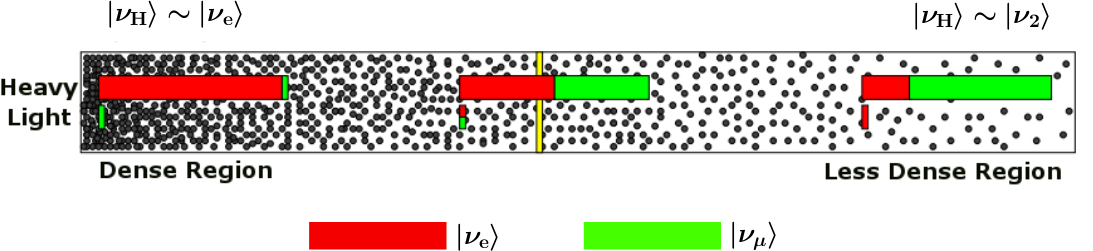
\includegraphics[width=0.9\textwidth]{assets/msw-and-density.png}
% \caption*{Yellow bar is the resonance point. Red: $\ket{\nu_e}$. Green: $\ket{\nu_\mu}$. Adapted from Smirnov, 2003.}
% \end{figure}
%
%
%
% \end{frame}
%
%
%
%
%
%
% \begin{frame}{MSW Effect}
%
%
% Suppose $\omega_{\mathrm v} = (m_2^2 - m_1^2)/2E <0$,
%
% \begin{equation*}
%     \mathbf{H} = \colorbox{blue!50}{$
%     -\frac{\omega_{\mathrm{v}}}{2}\begin{pmatrix} -\cos 2\theta_{\mathrm{v}} & \sin 2 \theta_{\mathrm{v}} \\ \sin 2\theta_{\mathrm{v}} & \cos 2\theta_{\mathrm{v}}  \end{pmatrix}
%     $}
%              \colorbox{red!50}{$
%             + \sqrt{2}G_{\mathrm{F}} n_{\mathrm{e}}(x) \begin{pmatrix}
%             1 & 0 \\
%             0 & 0
%             \end{pmatrix}
%             $}
% \end{equation*}
%
% \centering
% $\big\downarrow$
%
% \begin{equation*}
%     \mathbf{H} =
%     \left(
%     %\colorbox{blue!20}{$
%      \frac{-\omega_{\mathrm{v}}}{2} \cos 2\theta_{\mathrm{v}}
%     % $} \colorbox{red!20}{$
%     + \frac{\lambda(x)}{2}
%     % $}
%     \right) \boldsymbol{\sigma_3}
%     % \colorbox{blue!20}{$
%             - \frac{\omega_{\mathrm v}}{2}\sin 2\theta_{\mathrm v} \boldsymbol{\sigma_1}
%      %       $}
% \end{equation*}
%
% \end{frame}


%%%%%%%%%%%%%%%%%%%%%%%%%%%%%%%%%%%%%%%%%%%%%%%%%%%%%%%%%%%%%%%%%%
%%%%%%%%%%%%%%%%%%%% Stimulated Effect/Multi-frequency stimulation %%%%%%%%%%%%%%%
\subsection{Neutrino Oscillations in Matter and Rabi Oscillations}

\begin{frame}{Supernova Matter Density Profile}

\begin{tcolorbox}%[title=Why Do We Care]

Astrophysical environments: supernovae, accretion disks etc

\end{tcolorbox}

\begin{figure}
    \centering
    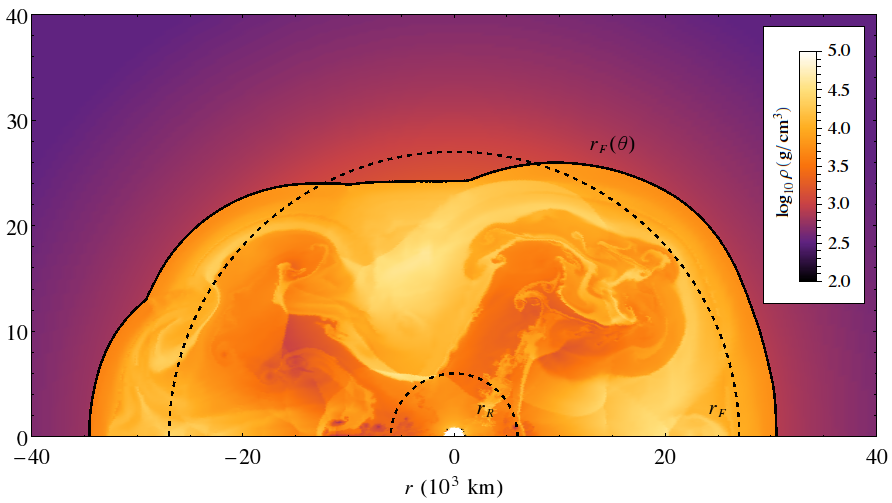
\includegraphics[height=0.5\textheight]{assets/supernova-shock-turbulence.png}
    \caption*{Supernova shock and turbulence. E. Borriello, et al  (2014)}
    %https://inspirehep.net/record/1262293?ln=en
    % arXiv: 1310.7488
    % 2seconds
\end{figure}



\end{frame}










\begin{frame}{Neutrino Flavor Conversions in Matter}







\begin{equation*}
    \lambda(x) = \lambda_0\only<2>{ + A \cos(k x )}
\end{equation*}



\only<1>{
\begin{figure}
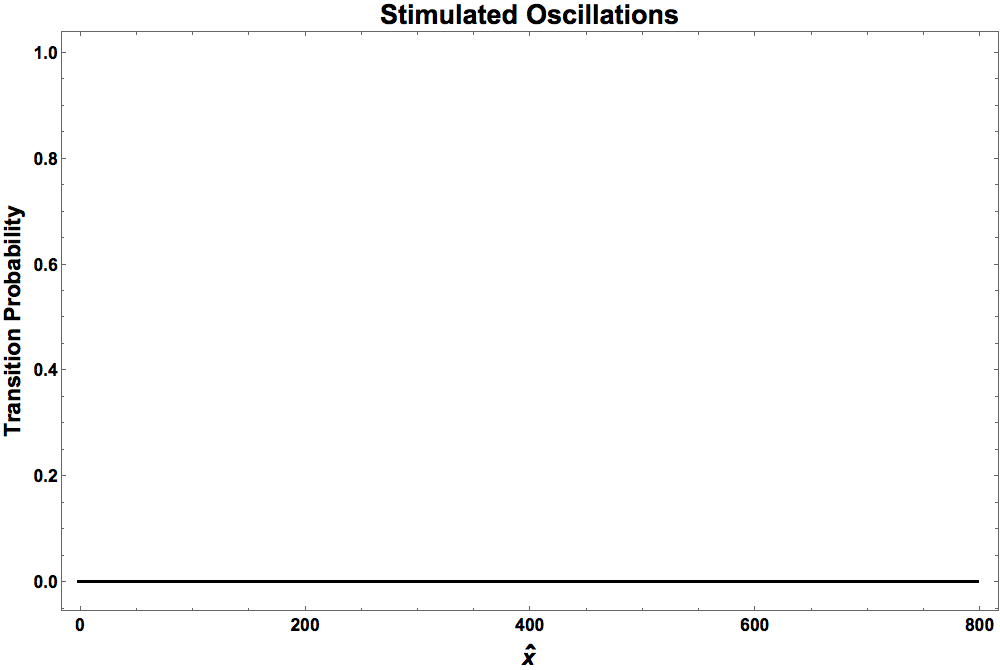
\includegraphics[width=0.8\textwidth]{assets/stimulated-oscillation-phenomenon-0.png}
\end{figure}
}




\only<2>{
\begin{figure}
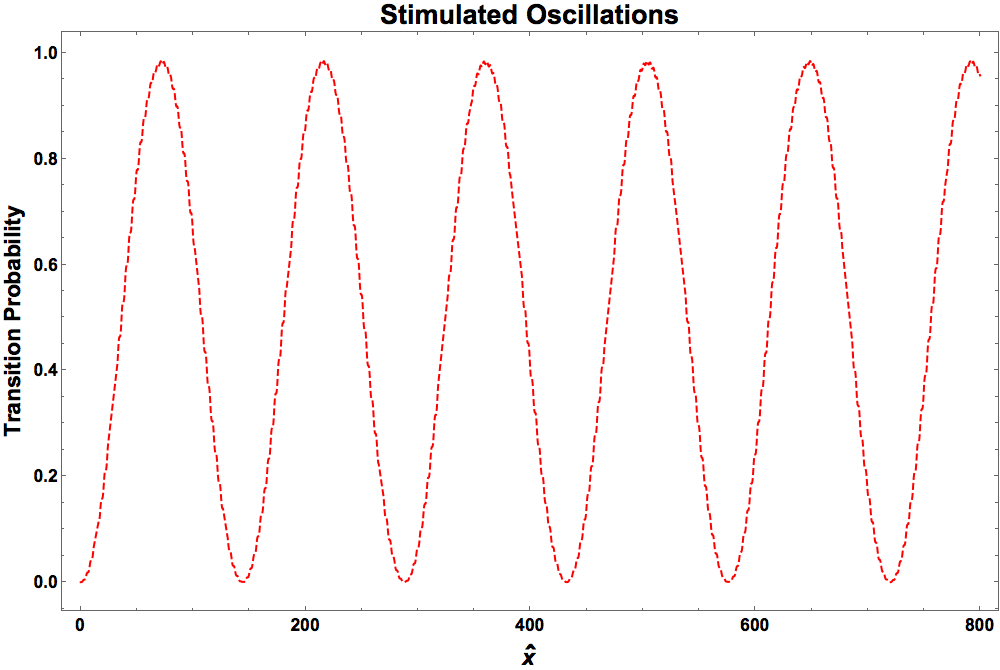
\includegraphics[width=0.8\textwidth]{assets/stimulated-oscillation-phenomenon.png}
%stimulated-neutrino-oscillations-kneller.png}
%\caption*{Stimulated oscillations. $\lambda(x) = \lambda_0 +  A \cos (k x)$
%with $\hat x = \omega_{\mathrm m} x $, $A=0.1\omega_{\mathrm m}$, $k=0.995\omega_{\mathrm m}$, $\theta_{\mathrm{m}}=\pi/6$
%}
\end{figure}
}


\only<1>{
\centering
Transition probabilities between mass states in matter.\newline
}

\only<2>{
{\small
P. Krastev and A. Smirnov (1989); A. Friedland et al (2006); J. Kneller et al (2013); K. Patton et al (2014);
}

\begin{textblock*}{100pt}(280pt,10pt)
   $A=0.1\omega_{\mathrm m}$\\ $k=0.995\omega_{\mathrm m}$\\ $\theta_{\mathrm{m}}=\pi/6$
\end{textblock*}

}


\end{frame}












%%%%%%%%%%%%%%%%%%%%%%%%%%%%%%%%
% Intuitive Demonstration BEGIN
%%%%%%%%%%%%%%%%%%%%%%%%%%%%%%%%







\begin{frame}{Rabi Oscillations}
\setbeamercovered{invisible}




\only<1,5>{

\begin{tcolorbox}[title=Rabi Oscillations,sidebyside]

  \begin{figure}
      \centering
      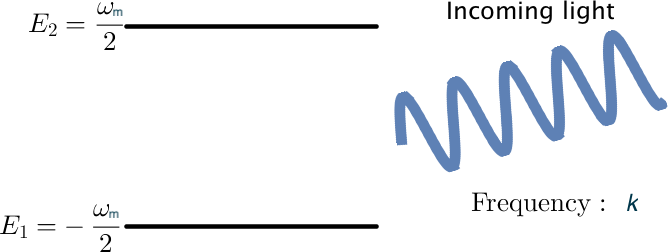
\includegraphics[width=\textwidth]{assets/rabi-diagram.png}
  \end{figure}

  \tcblower

  Hamiltonian

  \begin{equation*}
      -\frac{\omega_{\mathrm m}}{2} \sigma_3 - \frac{\alpha}{2} \begin{pmatrix}
      0 & e^{ikt}\\
      e^{-ikt} & 0
      \end{pmatrix}
  \end{equation*}

\end{tcolorbox}

% \begin{columns}[T]
%    \begin{column}{0.6\textwidth}
%       \begin{tcolorbox}[title=Scheme]
%    \begin{figure}
%        \centering
%        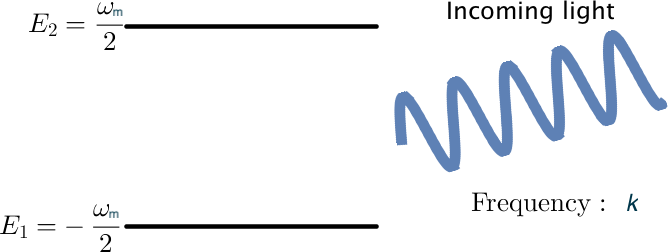
\includegraphics[width=\textwidth]{assets/rabi-diagram.png}
%    \end{figure}
%    \end{tcolorbox}
%
%
%    \end{column}%
% \begin{column}{0.4\textwidth}
% \begin{tcolorbox}[title=Rabi Oscillation]
%
% Hamiltonian
%
% \begin{equation*}
%     -\frac{\omega_{\mathrm m}}{2} \sigma_3 - \frac{\alpha}{2} \begin{pmatrix}
%     0 & e^{ikt}\\
%     e^{-ikt} & 0
%     \end{pmatrix}
% \end{equation*}
% \end{tcolorbox}
%
% \end{column}%
% \end{columns}



}


\only<2-3>{



\begin{columns}[T]
\begin{column}<2-3>{0.5\textwidth}

\centering
Static Frame

\begin{equation*}
    \vec H_3 = \omega_{\mathrm m}\begin{pmatrix}
    0 \\
    0\\
    1
    \end{pmatrix}, \vec H_+ = \alpha  \begin{pmatrix}
    \cos( kt) \\
    -\sin(kt)\\
    0
    \end{pmatrix}
\end{equation*}

\begin{figure}
    \centering
    \includegraphics[width=0.8\textwidth]{assets/rabi-isospin-static-frame}
\end{figure}


\end{column}%
\begin{column}<3>{0.5\textwidth}

\centering
Corotating Frame

\begin{equation*}
    \vec H'_3 = (\omega_{\mathrm m} - k)\begin{pmatrix}
    0 \\
    0\\
    1
    \end{pmatrix}, \vec H'_+ = \alpha  \begin{pmatrix}
    1 \\
    0\\
    0
    \end{pmatrix}
\end{equation*}

\begin{figure}
    \centering
    \includegraphics[width=0.8\textwidth]{assets/rabi-isospin-rotating-frame}
\end{figure}





\end{column}
\end{columns}


}




\only<4>{

\centering
Corotating Frame


\begin{equation*}
    \vec H'_3 = (\omega_{\mathrm m} - k)\begin{pmatrix}
    0 \\
    0\\
    1
    \end{pmatrix} = 0 \Rightarrow k=\omega_{\mathrm m}
\end{equation*}


\begin{figure}
    \centering
    \includegraphics[width=0.5\textwidth]{assets/rabi-isospin-rotating-frame-resonance}
\end{figure}


}



\only<5>{



Rabi formula

\begin{equation*}
    P_{1\to 2} = \frac{1}{1 + D^2} \sin^2 \left( \frac{\Omega_{\mathrm R}}{2} t \right).
\end{equation*}

Relative detuning

\begin{equation*}
    D = \left\vert\frac{\omega_{\mathrm m} - k}{\alpha} \right\vert.
\end{equation*}

Rabi frequency

\begin{equation*}
\Omega_{\mathrm R} = \lvert\alpha\rvert\sqrt{1+ D^2}
\end{equation*}



}


\end{frame}



\begin{frame}{Hamiltonian in Matter Basis}

\begin{textblock*}{10pt}(220pt,1pt)
\small
\begin{equation*}
\begin{pmatrix}
\psi_e\\
\psi_\mu
\end{pmatrix} = \begin{pmatrix}
\cos \theta_m & \sin\theta_m \\
-\sin \theta_m & \cos \theta_m
\end{pmatrix}\begin{pmatrix}
\psi_L\\
\psi_H
\end{pmatrix}
\end{equation*}

\end{textblock*}


% Matter profile
\begin{tcolorbox}[title=Matter Potential]
\begin{equation*}
    \lambda(x)  = \lambda_0 \only<2>{ + {\color{red}A\cos(k x)} }
\end{equation*}
\end{tcolorbox}


% Basis


\begin{tcolorbox}[title=Hamiltonian]

\only<2>{Background} matter basis:


\begin{equation*}
    \mathbf H = \frac{1}{2}\left( - \omega_{\mathrm{m}}
    \only<2>{
    + {\color{red}A\cos(kx)} \cos 2\theta_{\mathrm{m}}
    }
    \right) \boldsymbol{\sigma_3}
    \only<2>{
    - \frac{{\color{red}A\cos(kx) } }{2} \sin 2\theta_{\mathrm{m}} \boldsymbol{\sigma_1}
    }
\end{equation*}


\end{tcolorbox}






\end{frame}






\begin{frame}{Hamiltonian in Matter Basis}

% \begin{textblock*}{10pt}(240pt,1pt)
% \small
% \begin{equation*}
% \alpha = \frac{\sin2\theta_{\mathrm m}}{2}A
% \end{equation*}

% \end{textblock*}


Matter potential frequency

\begin{equation*}
    k\sim \omega_{\mathrm m}
\end{equation*}


\begin{align*}
    \mathbf {H} =\,& \frac{1}{2}\left( - \omega_{\mathrm{m}}
    +\cancel{
     \cos 2\theta_{\mathrm{m}}{A\cos(kx)} } \right) \sigma_3 - \frac{  \sin 2\theta_{\mathrm{m}
    }
    }{2}{A \cos(kx)}  \sigma_1 \\
    \to\, &  \omega_{\mathrm m}\begin{pmatrix}
    0\\
    0\\
    1
    \end{pmatrix} + \alpha \begin{pmatrix}
    \cos (kx)\\
    -\sin(k x)\\
    0
    \end{pmatrix}  + \only<1>{\alpha \begin{pmatrix}
    \cos (-kx)\\
    -\sin( - k x)\\
    0
    \end{pmatrix}
    }
    \only<2>{\cancel{\alpha \begin{pmatrix}
    \cos (-kx)\\
    -\sin( - k x)\\
    0
    \end{pmatrix}
    }
    }
\end{align*}

\begin{equation*}
\alpha = \frac{\sin2\theta_{\mathrm m}}{2}A
\end{equation*}







\end{frame}



\begin{frame}{Rabi Formula Works}


% \begin{textblock*}{10pt}(230pt,-1pt)
% {\tiny
% \begin{equation*}
% \vec H \sim  \omega_{\mathrm m}\begin{pmatrix}
%     0\\
%     0\\
%     1
%     \end{pmatrix} + \alpha \begin{pmatrix}
%     \cos (kx)\\
%     -\sin(k x)\\
%     0
%     \end{pmatrix}
% \end{equation*}
% }
% \end{textblock*}

\begin{tcolorbox}[colback=white]
\begin{figure}
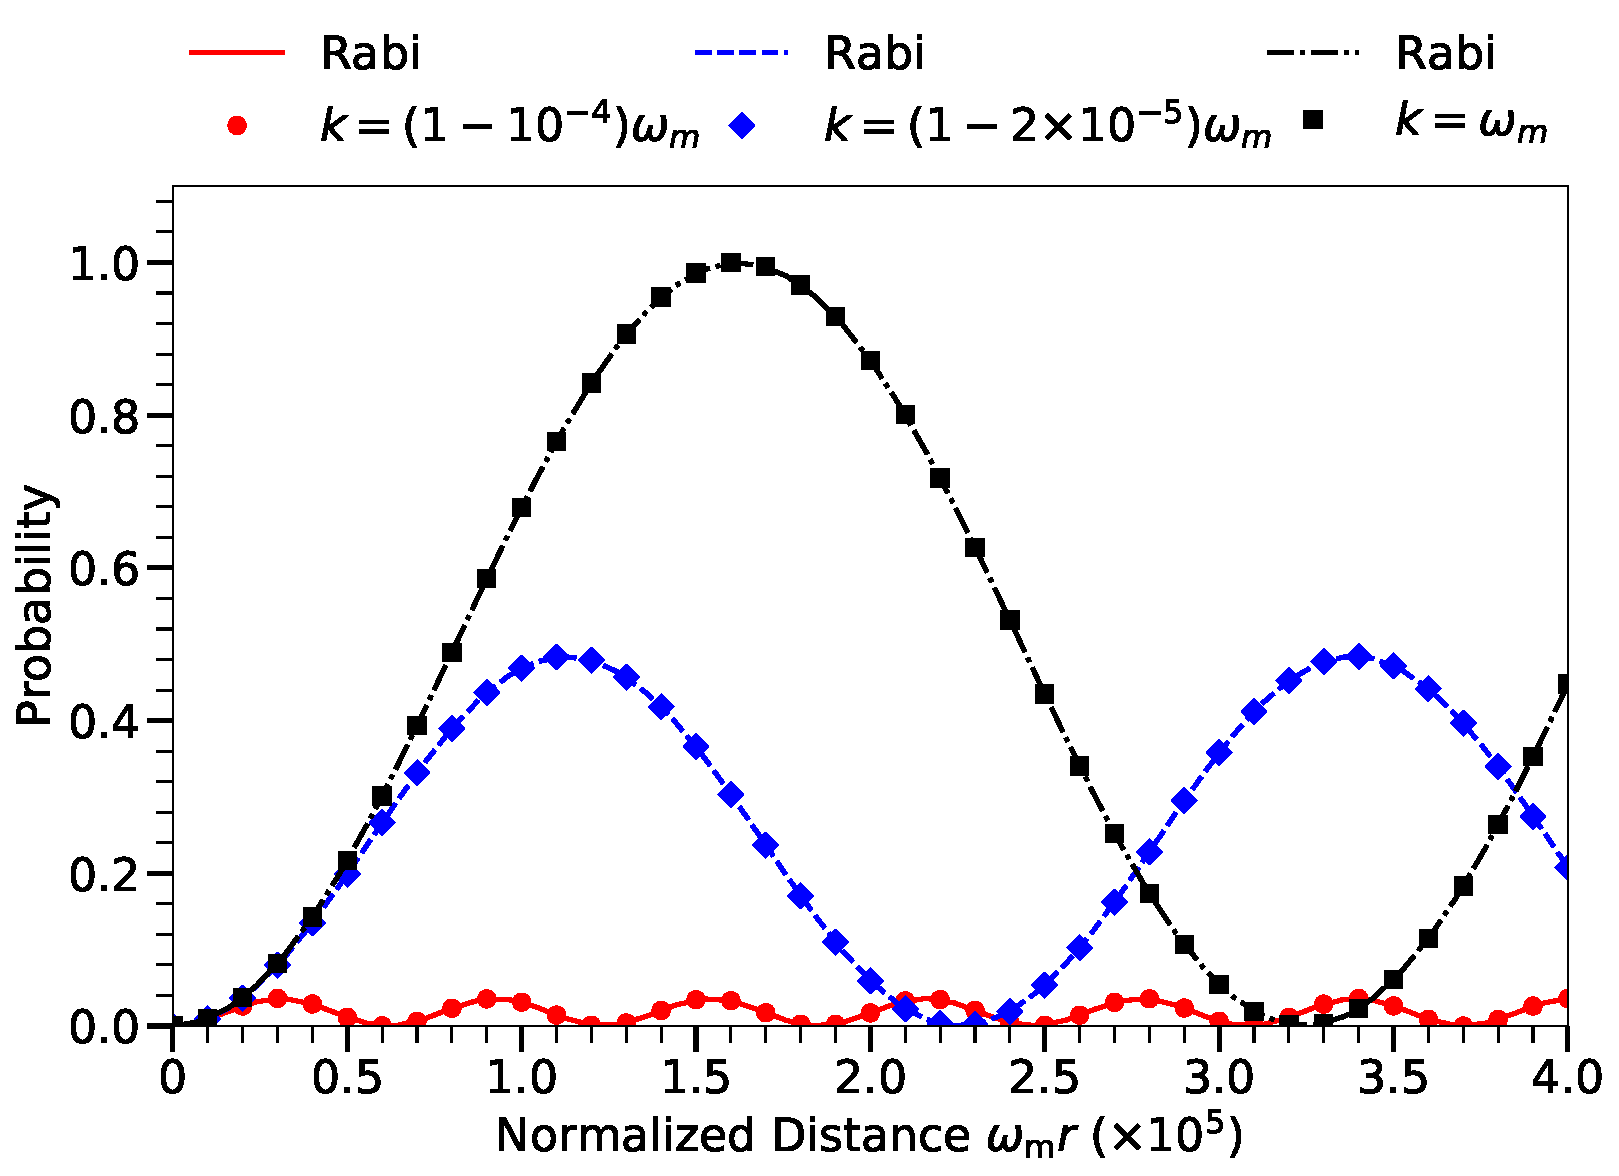
\includegraphics[width=0.9\textwidth]{assets/rabiOscillationsNeutrinoCoincidence-single-frequency-with-legend}
%stimulated-neutrino-oscillations-kneller.png}
\caption*{
\color{black}Transition between two mass states in background matter potential $\lambda_0$; $A_1 = -10^{-4}\omega_{\mathrm m}$
%\\
% Lines: Rabi formula\\
% \blacksquare : {\color{black}$k=\omega_{\mathrm m}$} \\
% : {\color{blue}$k=(1-2\times 10^{-5})\omega_{\mathrm m}$} \\
% {\tikz\draw[red,fill=red] (0,0) circle (.5ex);} : {\color{red}$k=(1-10^{-4})\omega_{\mathrm m}$}
}
\end{figure}
\end{tcolorbox}

\end{frame}





\begin{frame}{Single Frequency Matter Potential Revisited}

We have been making approximations.


\begin{align*}
    \mathbf {H} =\,& \frac{1}{2}\left( - \omega_{\mathrm{m}}
    +\cancel{
     \cos 2\theta_{\mathrm{m}}{A\cos(kx)} } \right) \sigma_3 - \frac{  \sin 2\theta_{\mathrm{m}
    }
    }{2}{A \cos(kx)}  \sigma_1 \\
    \to\, &  \omega_{\mathrm m}\begin{pmatrix}
    0\\
    0\\
    1
    \end{pmatrix} + \alpha \begin{pmatrix}
    \cos (kx)\\
    -\sin(k x)\\
    0
    \end{pmatrix}  + \cancel{\alpha \begin{pmatrix}
    \cos (-kx)\\
    -\sin( - k x)\\
    0
    \end{pmatrix}
    }
\end{align*}


\end{frame}



% \subsection{Rabi Basis }



\begin{frame}{Rabi Basis}



\begin{tcolorbox}[title=Hamiltonian in Background Matter Basis]
    \begin{equation*}
    \mathbf {H} = \frac{1}{2}\left( - \omega_{\mathrm{m}} + {\color{red}A\cos(kx)} \cos 2\theta_{\mathrm{m}} \right) \boldsymbol{\sigma_3} - \frac{  {\color{red}A\cos (kx)}  }{2} \sin \theta_{\mathrm{m}} \boldsymbol{\sigma_1}.
\end{equation*}
\end{tcolorbox}


\begin{tcolorbox}[title=A Better Basis]


Define Rabi basis %\{$\ket{\tilde\nu_{\mathrm{L} }}$,$\ket{\tilde\nu_{\mathrm{H} }}$\}
in which the wave function is related to wave function in background matter basis
%\{$\ket{\nu_{\mathrm{L} }}$,$\ket{\nu_{\mathrm{H} }}$\}
through

\begin{equation*}
    \begin{pmatrix}
    \psi_{\mathrm{L} } \\
    \psi_{\mathrm{H} }
    \end{pmatrix} = \begin{pmatrix}
     e^{-i \eta (x)} & 0 \\  0 & e^{i \eta (x)}
    \end{pmatrix}\begin{pmatrix}
    \tilde\psi_{\mathrm{L} }\\
    \tilde\psi_{\mathrm{H} }
    \end{pmatrix},
\end{equation*}

where

\begin{equation*}
    \eta(x) - \eta(0) = \frac{\cos 2\theta_{\mathrm{m}}}{2} \int_0^x {\color{red}A\cos(k \tau)} d\tau.
\end{equation*}

\end{tcolorbox}



\end{frame}














\begin{frame}{Single Frequency Matter Potential}
% \setbeamercovered{invisible}



\begin{equation*}
\lambda(x) = \lambda_0 +  A \cos(k x )
\end{equation*}


\begin{tcolorbox}[title=Hamiltonian in Rabi Basis]

The Hamiltonian


\begin{equation*}
\mathbf{\widetilde H}= -\frac{\omega_{\mathrm m}}{2}\sigma_3 + \sum_{n=-\infty}^{\infty} \begin{pmatrix}
0 & \frac{1}{2}  \alpha_n e^{i  {\color{red} (n k) } x}\\
\frac{1}{2}  \alpha_n^* e^{ -i  {\color{red} (n k) } x} & 0
\end{pmatrix}
\end{equation*}


where $\alpha_n =  - (-i)^n  {\color{red}n  k} \tan 2\theta_{\mathrm{m}}  J_n ( A \cos 2\theta_{\mathrm{m}} / k )$.


\end{tcolorbox}







\begin{tcolorbox}
\centering
Map neutrino oscillations in single frequency matter potential to Rabi oscillations with many driving potentials.
\end{tcolorbox}

\pause
\begin{tcolorbox}
\centering
Resonance condition for each mode: $nk=\omega_{\mathrm m}$
\end{tcolorbox}




\end{frame}



\begin{frame}{Rabi Oscillations With Multiple Driving Frequencies}




Relative detuning for two driving potentials, $\alpha_1,k_1$ and $\alpha_2, k_2$

\begin{equation*}
D' =  \left\vert \frac{\omega_{\mathrm m} - k_1 }{\alpha_1} + \frac{\alpha_2^2}{2\alpha_1(\omega_{\mathrm m}-k_2)} \right\vert
\end{equation*}

Amplitude

\begin{equation*}
   \frac{1}{1+D'^2}
\end{equation*}

\end{frame}


\begin{frame}{Rabi Oscillations With Multiple Driving Frequencies}

% \begin{textblock*}{100pt}(260pt,10pt)
% % \textblockcolour{black}
% \tiny
% \begin{equation*}
% D' =  \left\vert \frac{\omega_{\mathrm m} - k_1 }{\alpha_1} + \frac{\alpha_2^2}{2\alpha_1(\omega_{\mathrm m}-k_2)} \right\vert
% \end{equation*}
% \end{textblock*}


\begin{figure}
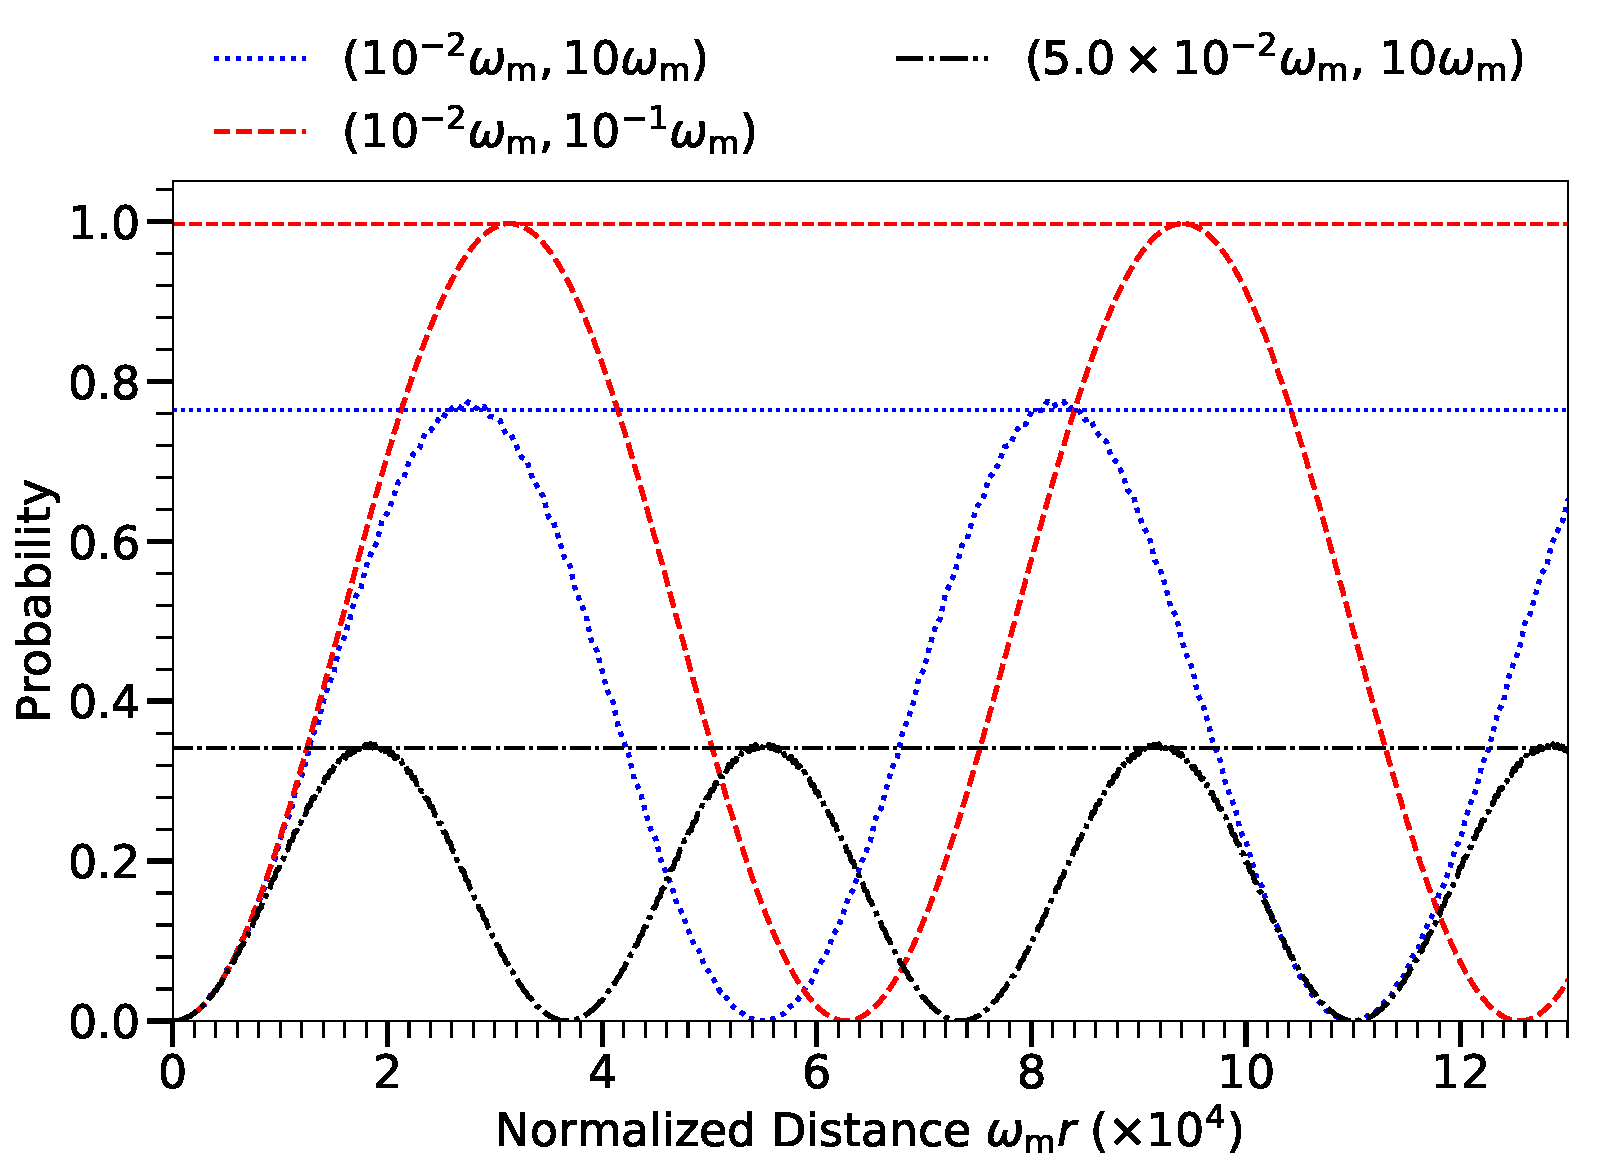
\includegraphics[width=0.9\textwidth]{assets/interference-reduction-slide-with-legend}
\caption*{$A_1=10^{-4}\omega_{\mathrm m}$, $k_1= \omega_{\mathrm m}$; Legend shows $(A_2, k_2)$; Grid lines: amplitude predicted using $1/(1+D'^2)$
}
\end{figure}


% Dashed line, dotted line, dash-dotted line, and solid line are for $A_2=10^{-2}\omega_{\mathrm{m}}$, $k_2=10\omega_{\mathrm m}$, $A_2=10^{-2}\omega_{\mathrm{m}}$, $k_2=10^{-1}\omega_{\mathrm m}$, $A_2=5.0\times 10^{-2}\omega_{\mathrm{m}}$, $k_2=10\omega_{\mathrm m}$, and $A_2=5\times 10^{-2}\omega_{\mathrm{m}}$, $k_2=10^{-1}\omega_{\mathrm m}$

% {\tiny
% \vspace{-15pt}
% \begin{center}
%     \begin{tabular}{c|c|c|c}
%     \multicolumn{4}{c}{ $A_2$, $k_2$ values} \\
%     \hline
%        Dashed  &  dotted & dash-dotted & solid \\
%        $10^{-2}\omega_{\mathrm{m}}$, $10\omega_{\mathrm m}$  &  $10^{-2}\omega_{\mathrm{m}}$, $10^{-1}\omega_{\mathrm m}$  & $5.0\times 10^{-2}\omega_{\mathrm{m}}$, $10\omega_{\mathrm m}$  & $5\times 10^{-2}\omega_{\mathrm{m}}$, $10^{-1}\omega_{\mathrm m}$
%     \end{tabular}
% \end{center}
% }

\end{frame}



\begin{frame}{Rabi Oscillations With Multiple Driving Frequencies}


%
% Consider $k_1=\omega_{\mathrm m}$
%
% \begin{equation*}
% D' =  \left\vert \frac{\alpha_2^2}{2\alpha_1(\omega_{\mathrm m}-k_2)} \right\vert
% \end{equation*}
%
% Amplitude reduces from 1 to 1/2 if
%
% \begin{equation*}
%     D'=1 \Rightarrow \alpha_{2,\mathrm C} \equiv \sqrt{ 2 \lvert \alpha_1 (k_2 - \omega_{\mathrm m}) \rvert }.
% \end{equation*}
%
%
% \vspace{2em}

\begin{tcolorbox}
Two driving frequencies $k_1$, and $k_2$, with amplitude $\alpha_1$, and $\alpha_2$

For $k_1 = \omega_{\mathrm m}$, survival of resonance requires

\begin{equation*}
    \lvert \alpha_2\rvert \ll  \alpha_{2,\mathrm C}\equiv\sqrt{ 2 \lvert \alpha_1 (k_2 - \omega_{\mathrm m}) \rvert }
\end{equation*}

\end{tcolorbox}






\end{frame}









\begin{frame}{Single Frequency Matter Potential}


\only<1->{

\begin{tcolorbox}
\begin{figure}
\centering
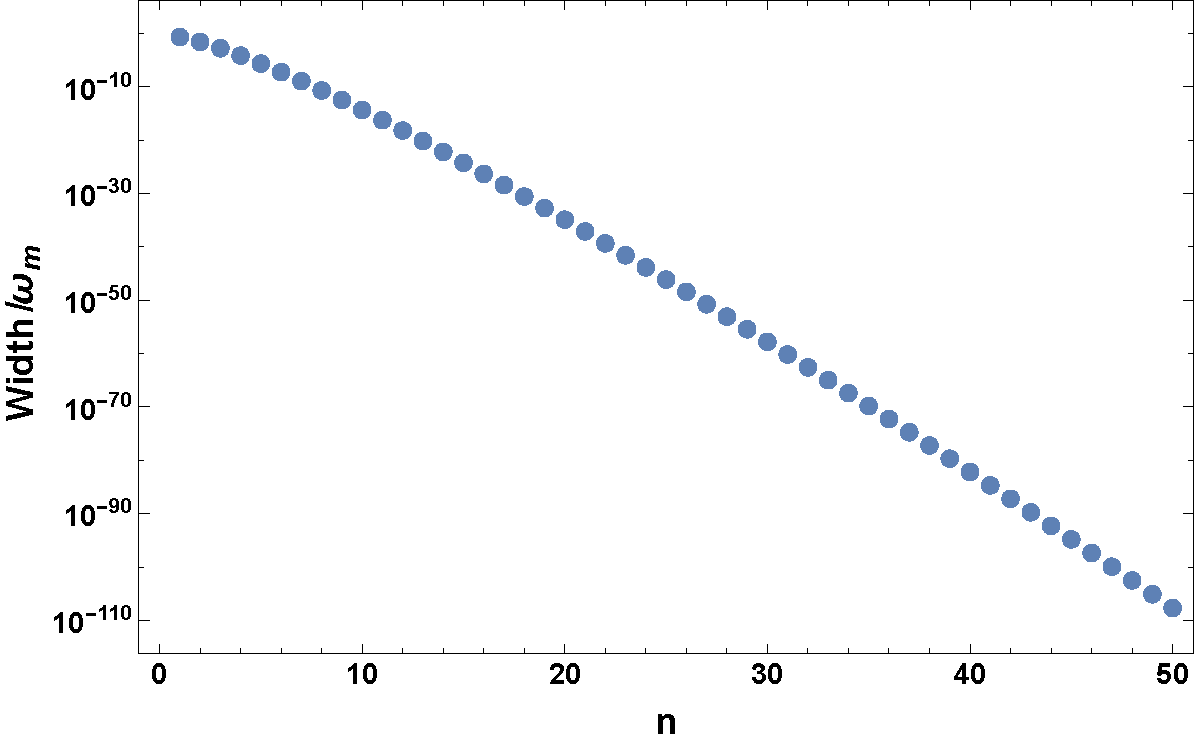
\includegraphics[width=0.95\textwidth]{assets/width-n}
\caption*{\color{black}Width of different modes given value of matter potential frequency $k$}
\end{figure}
\end{tcolorbox}
}

\only<2->{
\begin{textblock*}{280pt}(40pt,100pt)
\begin{tcolorbox}
   \centering
Higher modes are less important
\end{tcolorbox}
\end{textblock*}
}



\end{frame}



\begin{frame}<presentation:0>[noframenumbering]{Single Frequency Matter Potential}

Resonance conditions:

\begin{equation*}
    nk=\omega_{\mathrm m}
\end{equation*}

However, higher order resonances for n large usually have extremely small width.



\end{frame}



\subsection{Multiple Frequencies in Matter Potential}




\begin{frame}{Castle Wall Matter Potential}

\begin{tcolorbox}[opacityback=0, standard jigsaw, coltext=white]
  Rabi oscillation piscture also works for matter potential with multiple frequencies.
\end{tcolorbox}


\begin{columns}[T]
\begin{column}{0.5\textwidth}

\only<1,2, 3>{

\begin{figure}
    \centering
    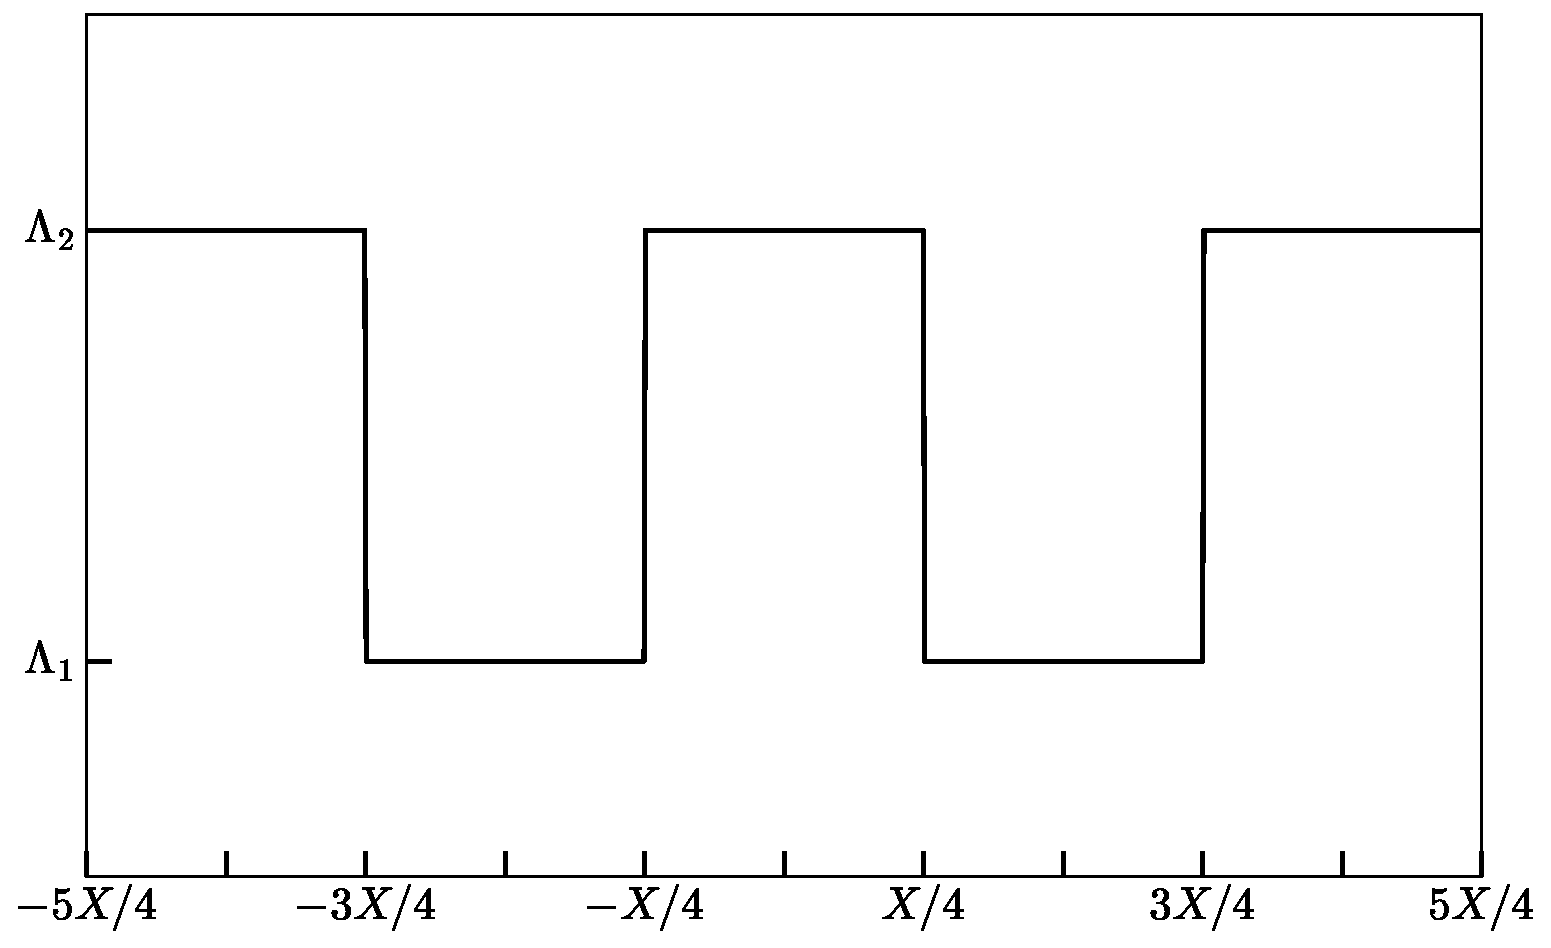
\includegraphics[width=\columnwidth]{assets/castlewall-profile}
    \caption*{Castle wall matter profile: \\ $\Lambda_2 =0.7\omega_{\mathrm v} \cos 2\theta_{\mathrm v} $ \\  $\Lambda_1 = 0.3\omega_{\mathrm v} \cos 2\theta_{\mathrm v}$  }
\end{figure}

% \begin{tcolorbox}[coltext=white, standard jigsaw, opacityback=0]
%    Density is smaller than MSW density requirement.
% \end{tcolorbox}

}

% \only<3>{
% \begin{table}
% \caption*{Relative detuning of each frequency.}
% \begin{tabular}{lll}
%  $\{n_1,n_2\}$  & $D'_{\{n_1,n_2\}}$   \\
% \hline \\
%  $\{1,0\}$ & $0$  \\
%  $\{1,0\}$ \& $\{-1,0\}$ &  $1.0\times 10^{-2}$ \\
%  $\{1,0\}$ \& $\{0,1\}$ &   $1.1\times 10^{-3}$  \\
%  $\{1,0\}$ \& $\{2,0\}$ &  $2.0\times 10^{-4}$
% \end{tabular}
% \end{table}

% }

\end{column}%
\begin{column}{0.5\textwidth}

\only<1,2>{
\small
\begin{equation*}
    \lambda(x)= \lambda_0 + \sum_1^\infty \lambda_n \cos (k_n x)
\end{equation*}

where

\begin{align*}
    \lambda_0 = & (\Lambda_1+\Lambda_2)/2 \\
    \lambda_n = & 2(-1)^n(\Lambda_1-\Lambda_2)/(2n\pi-\pi) \\
    k_n =& 2\pi (2n-1)/X
\end{align*}

}

\only<2>{
\begin{tcolorbox}
  Choose period $X =2\pi/\omega_{\mathrm m}$ so that
   \begin{equation*}
      k_1 = \omega_{\mathrm m}
   \end{equation*}
\end{tcolorbox}
}

\only<3>{
\begin{figure}
        % 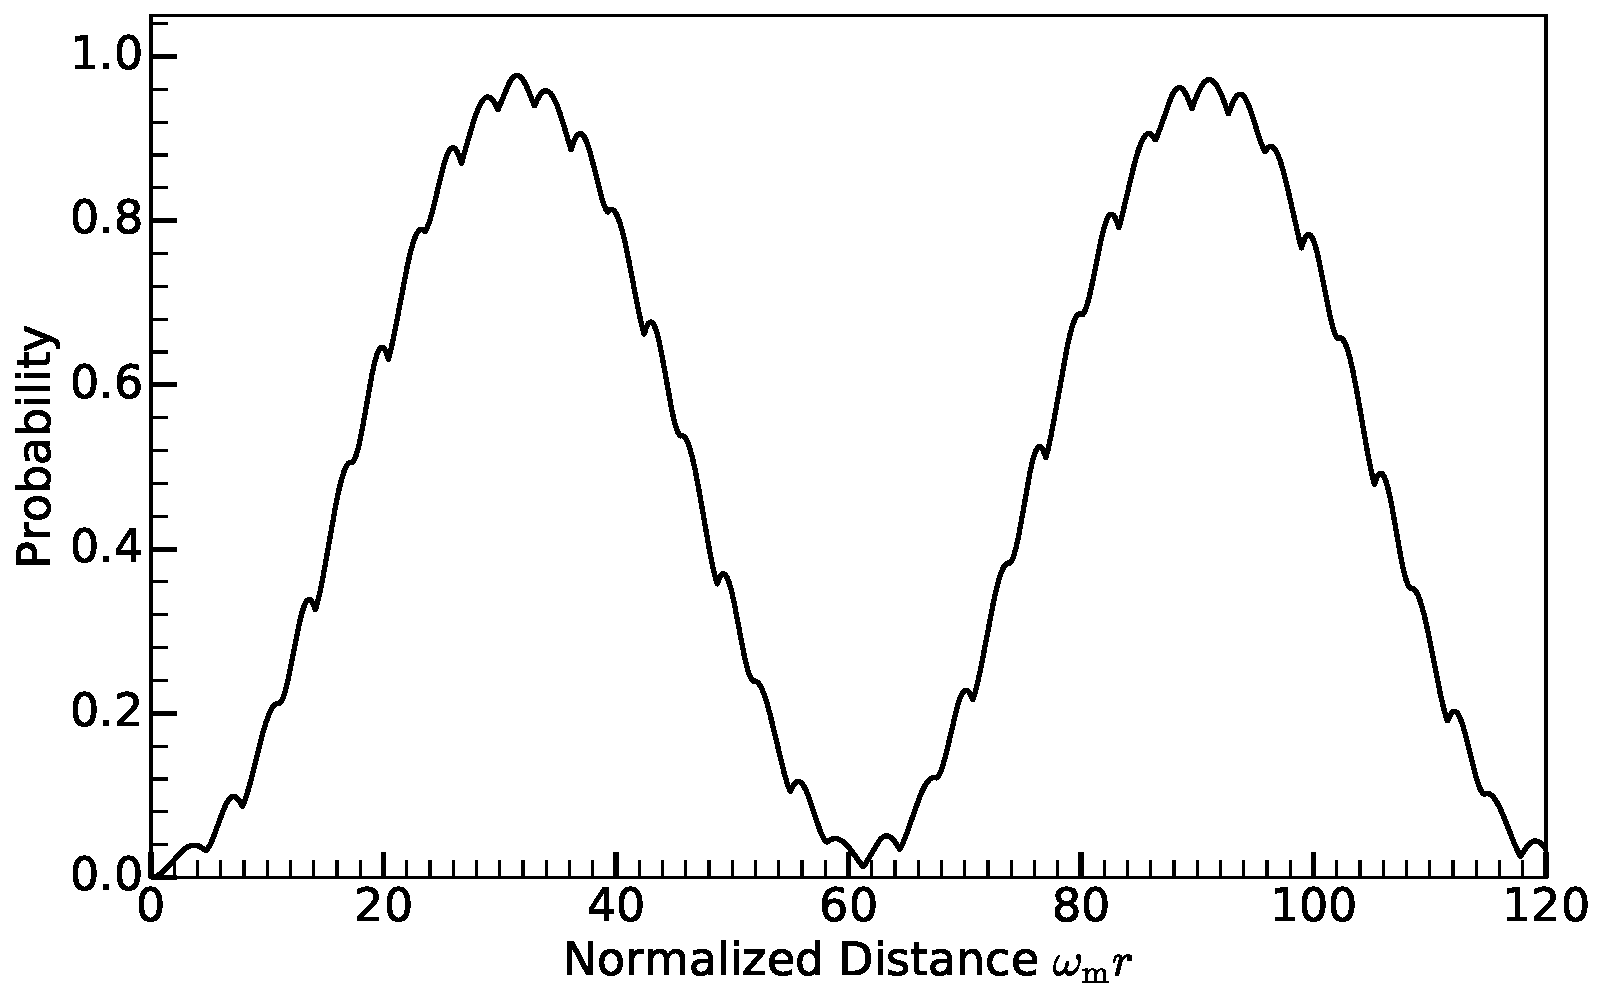
\includegraphics[width=\columnwidth]{assets/castle-wall-1}%
        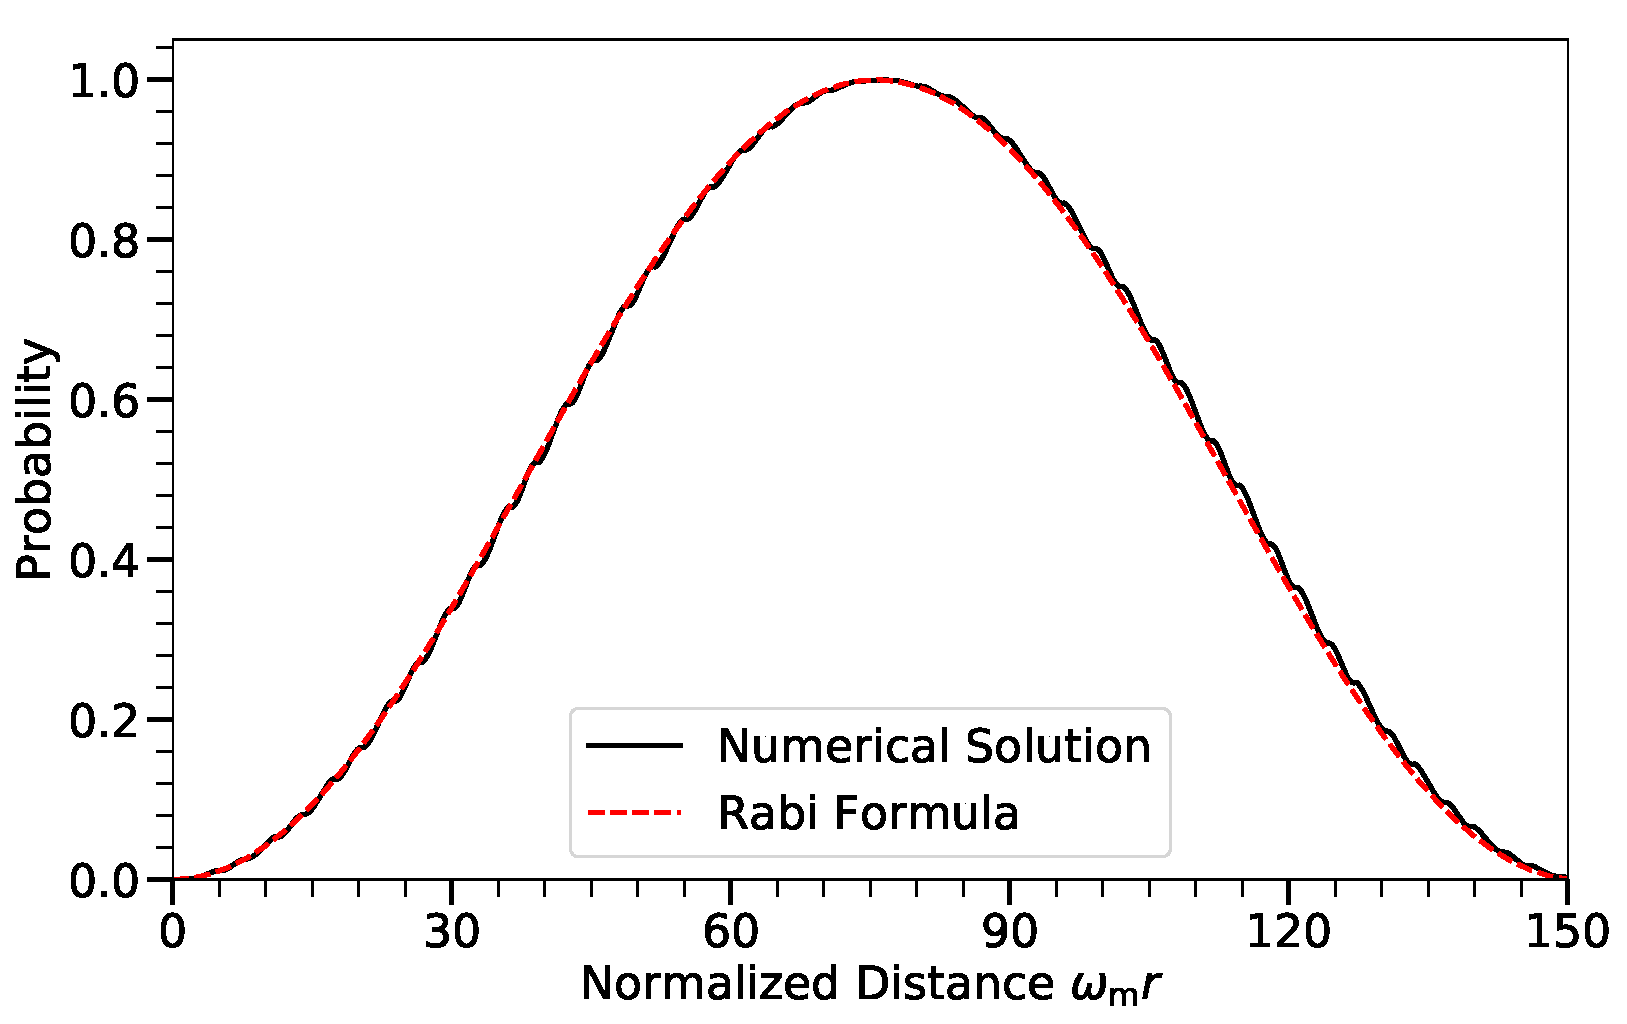
\includegraphics[width=\columnwidth]{assets/castle-wall-with-legend}%
     \caption*{Transition probability is a Rabi resonance with small variations due to higher orders.}
\end{figure}
}

\end{column}
\end{columns}




\end{frame}


\subsection{Summary of Neutrino Oscillations in Vacuum and Matter }


\begin{frame}{Summary of Neutrino Oscillations in Matter}


\begin{columns}[T]
\begin{column}{0.6\textwidth}

\begin{enumerate}[<+->]
\item
Vacuum oscillations: flavor states are not mass states.
\item
MSW resonance: matter potential cancels out the vacuum diagonal elements of the Hamiltonian.
\item
Neutrino oscillations in matter: variation in matter potential can cause resonances.

\item
In many cases neutrino oscillations in multi-frequency matter potential can be viewed as Rabi oscillations with few driving frequencies.
\end{enumerate}

\end{column}
\begin{column}{0.4\textwidth}

\only<1>{
\begin{figure}
    \centering
    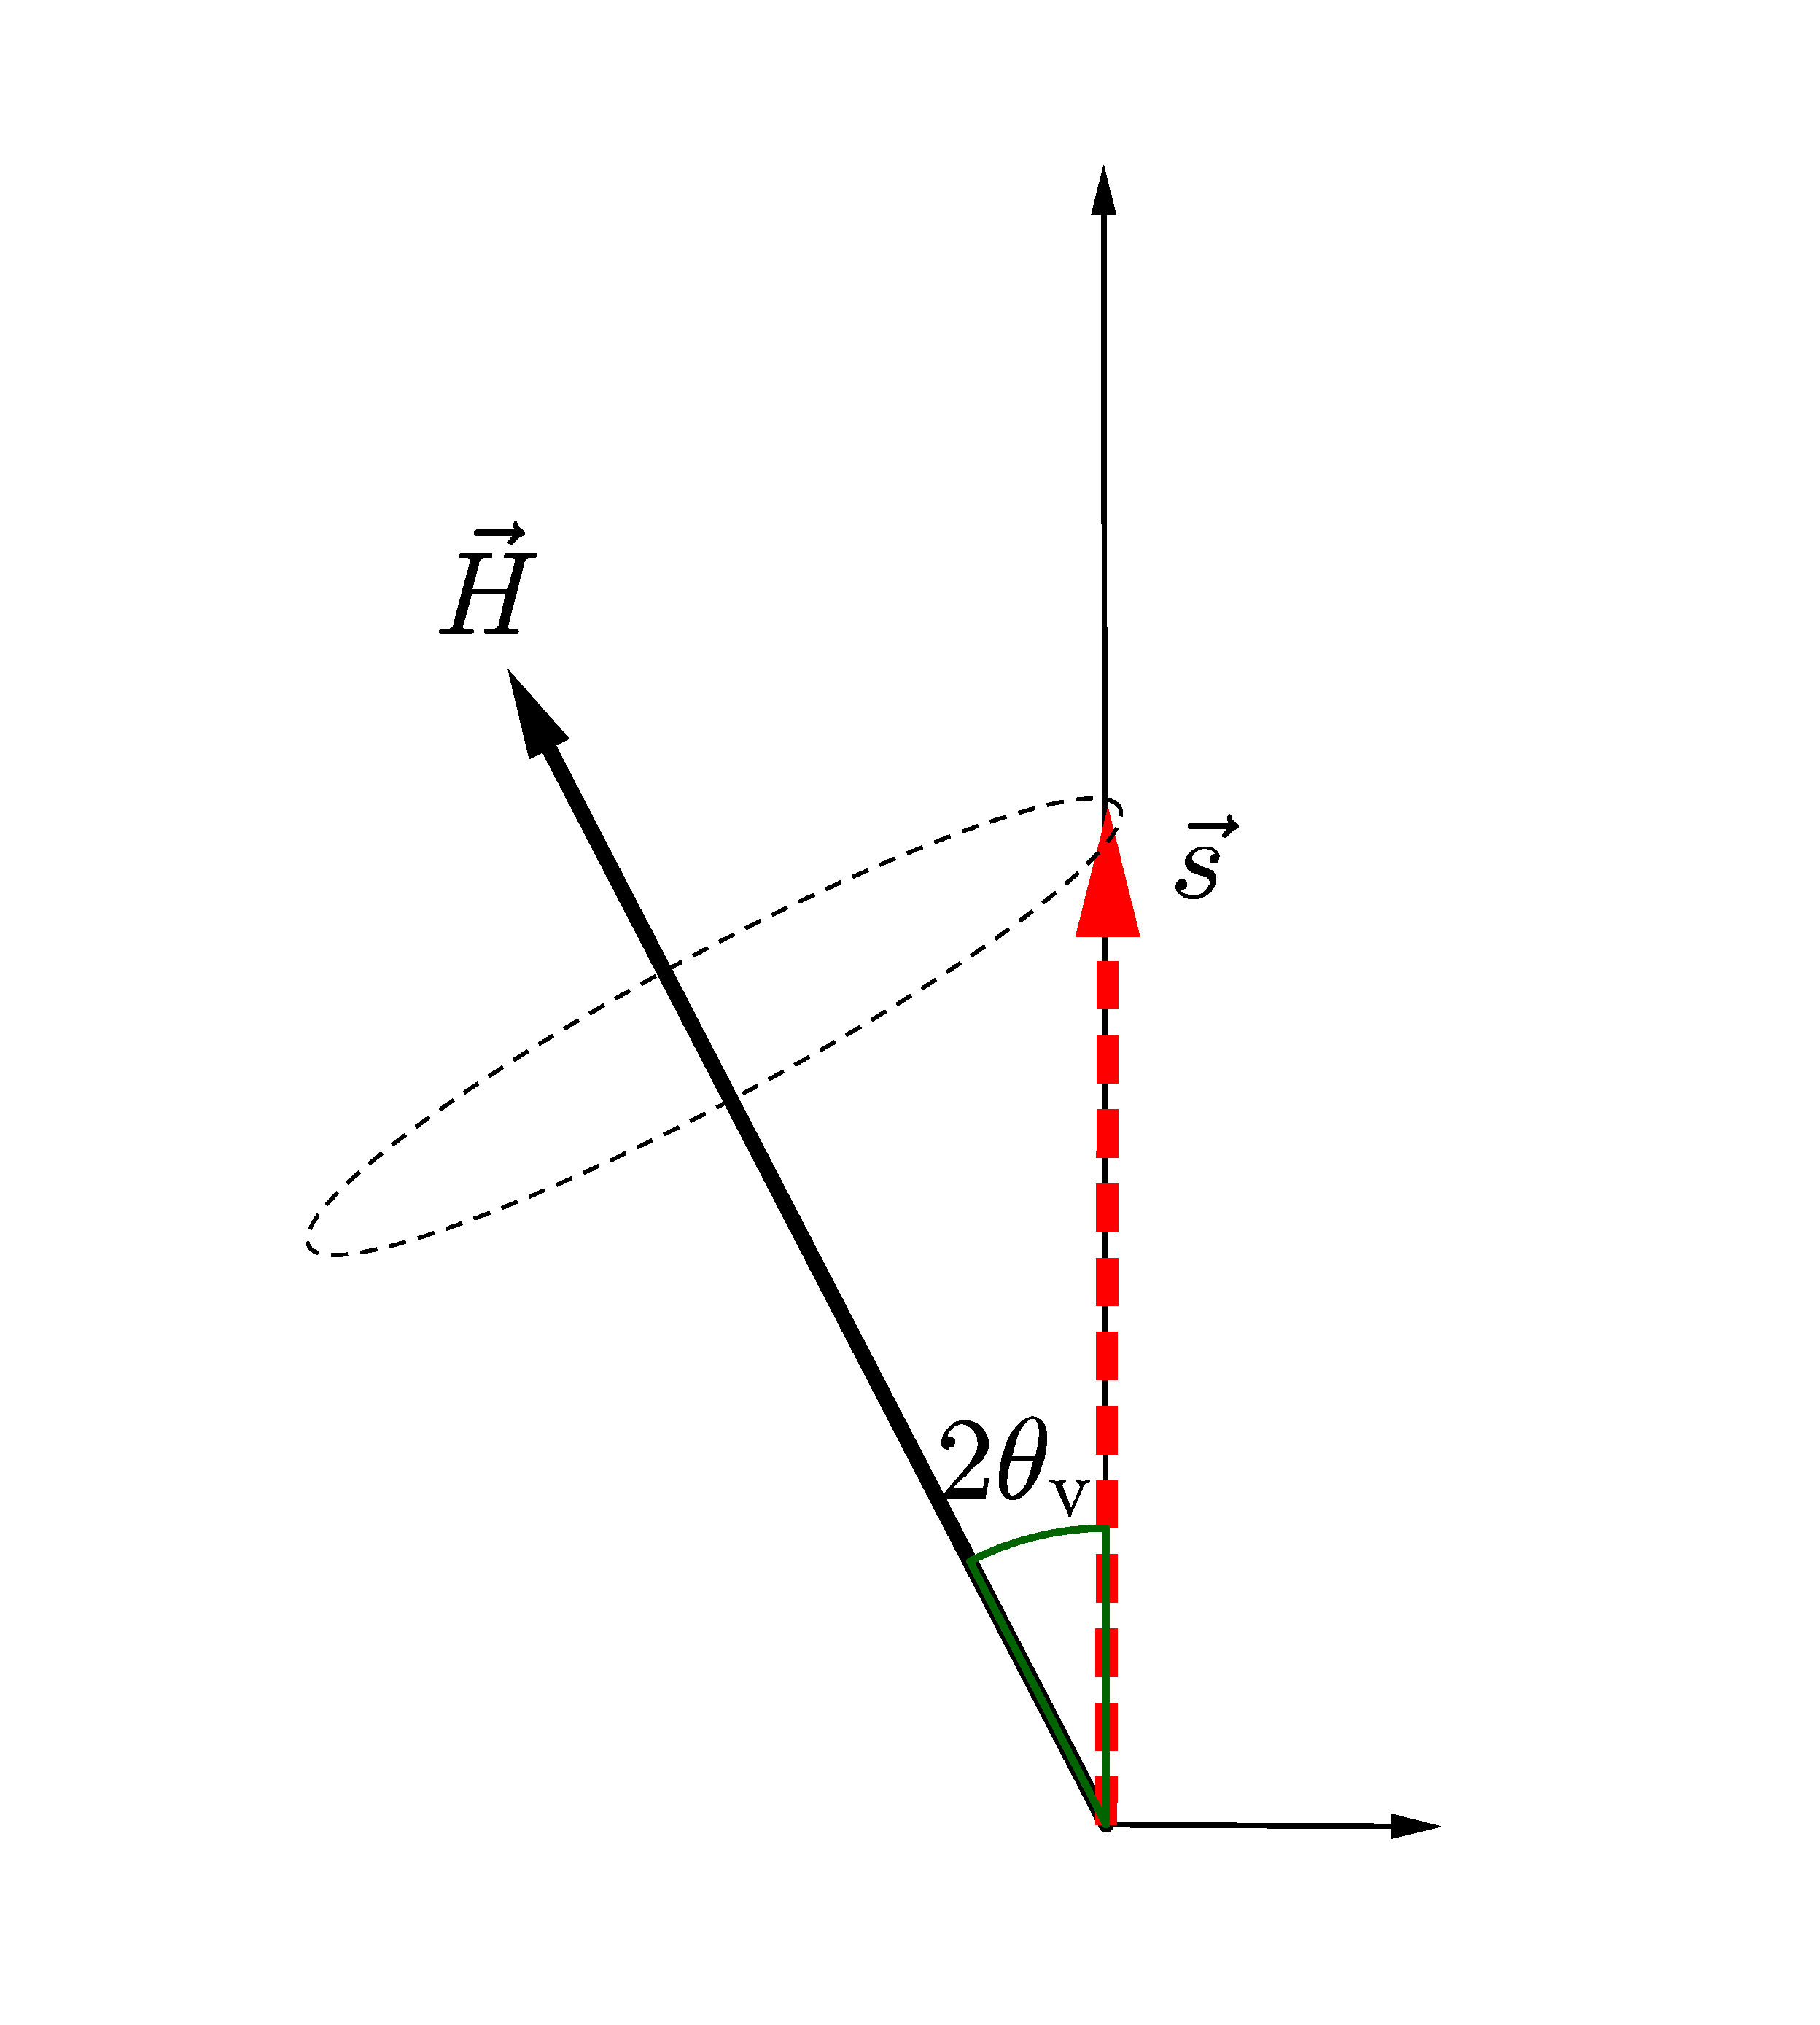
\includegraphics[width=0.9\textwidth]{assets/flavor-isospin-1}
\end{figure}
}

\only<2>{
\begin{figure}
    \centering
    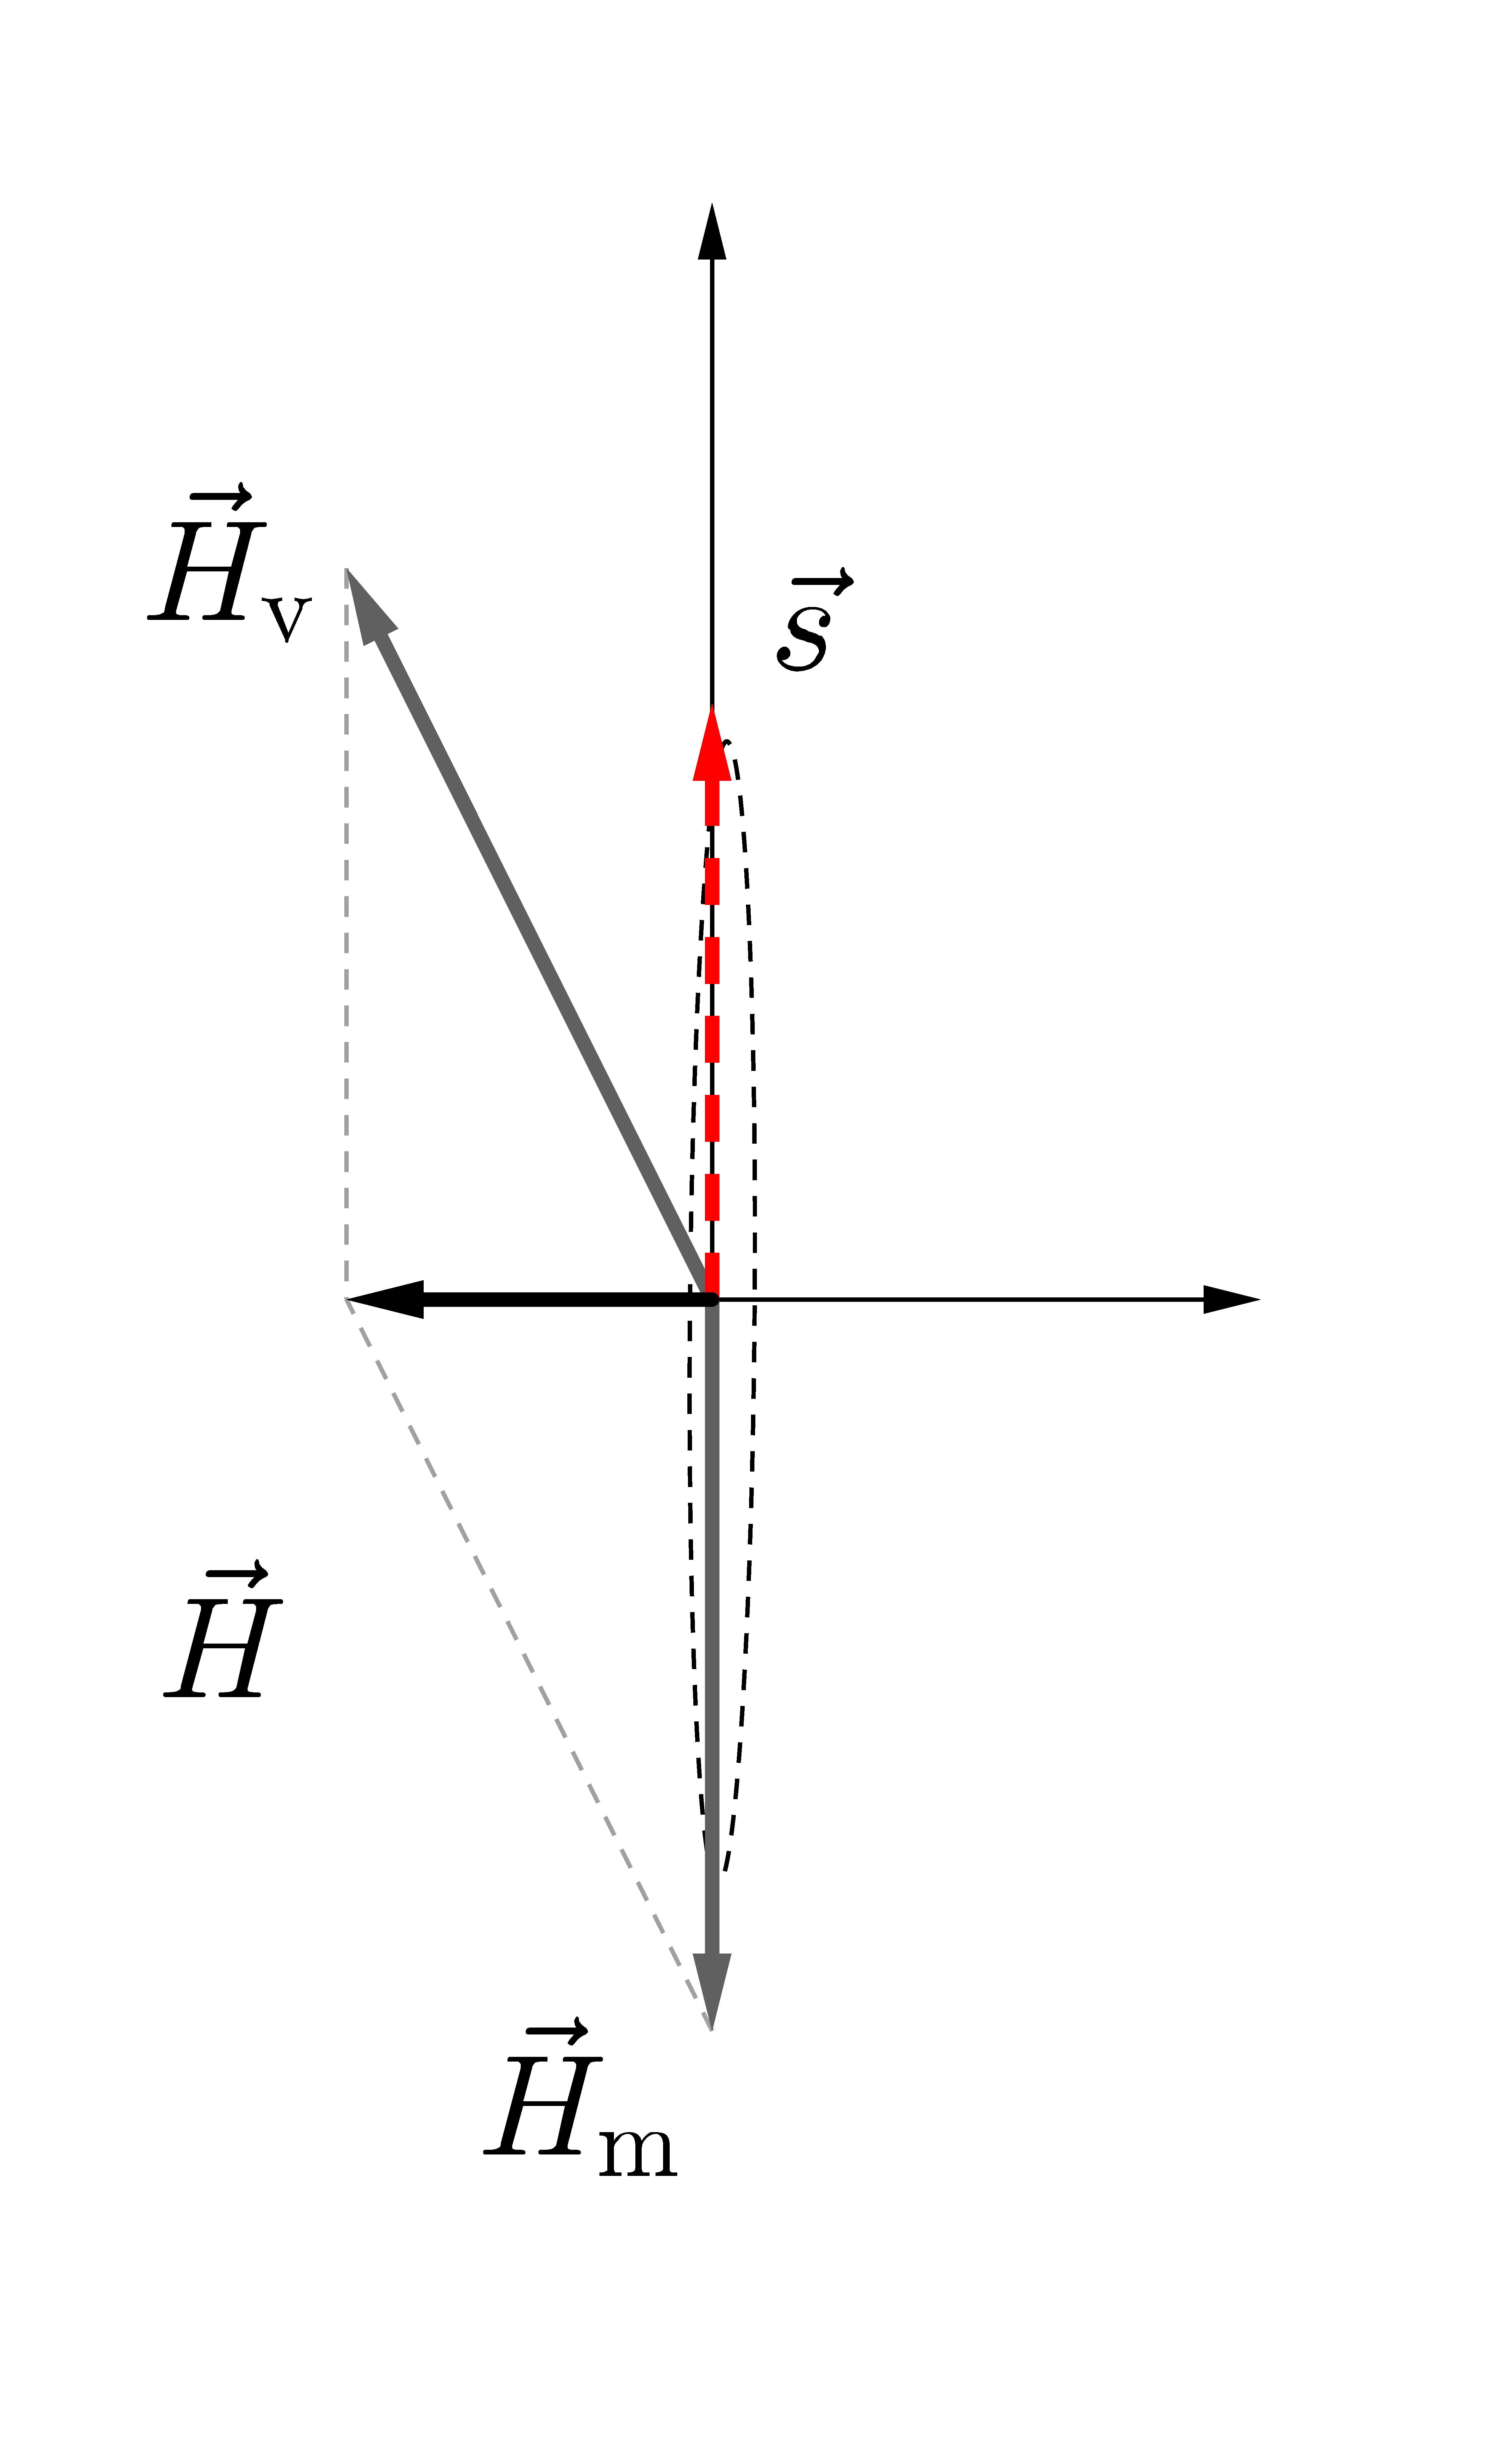
\includegraphics[width=0.9\textwidth]{assets/matter-effect-critical-density}
\end{figure}
}

\only<3>{
For matter potential

\begin{equation*}
\lambda(x) = \lambda_0 + A\cos(k x),
\end{equation*}

Resonance condition

\begin{equation*}
    n k = \omega_{\mathrm m}
\end{equation*}

}

\only<4>{


% \begin{equation*}
% \lvert \alpha_2\rvert \gg \alpha_{2,\mathrm C} \equiv \sqrt{ 2 \lvert \alpha_1 (k_2 - \omega_{\mathrm m}) \rvert }
% \end{equation*}


}

\end{column}
\end{columns}

\end{frame}
